\chapter{مفاهیم اولیه‌}\label{chapter2}

در این بخش به توضیح بیشتر مفاهیم معرفی شده (اینترنت اشیاء، رایانش ابری و بدون سرور) پرداخته شده، سپس پروژه‌ها و راه حل های موجود برای توسعه هر کدام از این محیط‌ها بررسی می‌شود.

\section{اینترنت اشیاء}

اینترنت اشیاء شبکه‌ای از دستگاه‌های هوشمند فیزیکی مانند لوازم خانگی، وسایل نقلیه، دستگاه های پوشیدنی و حسگرها است. این دستگاه‌ها \lr{Things} نامیده می‌شوند و از اینترنت برای برقراری ارتباط با یکدیگر استفاده می‌کنند. دستگاه‌های اینترنت اشیاء از نظر ماهیتی هوشمند، به هم پیوسته و محدود به منابع هستند. خانه هوشمند‌، کشاورزی‌، مراقبت‌های پزشکی‌ و سیستم حمل و نقل هوشمند برخی از زمینه‌هایی هستند که در آینده‌ نه چندان دور به دستگاه‌های اینترنت اشیاء متکی خواهند بود. به عنوان مثال، خودرو‌ی هوشمند از طریق ارتباط با خودروهای دیگر اطلاعات ترافیک را تجزیه و تحلیل می‌کند. در مثال دیگر پزشکان از طریق دستگاه‌های اینترنت اشیاء بر سلامتی بیماران نظارت می‌کنند. ارتباطات ذکر شده در بالا نیاز به اتصال بین دستگاه‌ها دارد و منجر به تولید حجم زیادی از داده‌ها می شود. با رشد اینترنت اشیاء، دنیایی در حال ایجاد است که میلیاردها دستگاه همه‌ی داده‌ها را جمع می‌کنند و از این داده‌ها می توان برای دستیابی به چیزی استفاده کرد که اگر همه این دستگاه‌ها به یکدیگر و اینترنت متصل نبودند، هیچگاه امکان پذیر نبود.

شکل \ref{IoT_explained} ارتباط بین انواع دستگاه‌های اینترنت اشیاء و \lr{gateway}، پروتکل‌های ارتباطی و ارتباط با بستر خدمات ابری را نشان می‌دهد. 

\begin{figure}[!h]
	\centering
	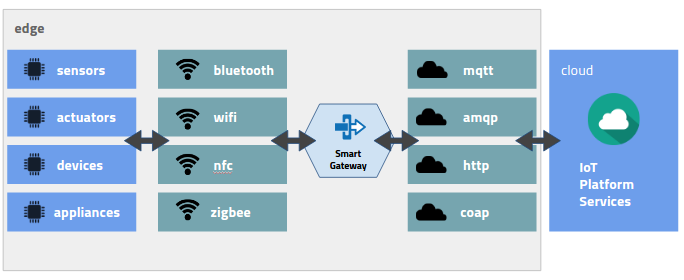
\includegraphics[height=7cm]{images/IoT_explained}
	\caption{ساختار شبکه‌ی اینترنت اشیاء}
	\label{IoT_explained}
\end{figure}

\newpage

دستگاه‌های اینترنت اشیاء ویژگی‌های بسیاری دارند که آن‌ها را از دستگاه‌های رایانشی قدیمی متمایز می‌کند. در ادامه این خصوصیات بررسی می‌شوند.

\begin{itemize}
	
	\item \textbf{تنوع زیاد:} دستگاه‌های اینترنت اشیاء در سخت‌افزار و قابلیت‌های مختلف متفاوت هستند. در نتیجه، یک شبکه اینترنت اشیاء شامل دستگاه‌های مختلف برای تعامل با یکدیگر است.
	
	\item \textbf{محدودیت منابع:} دستگاه‌های اینترنت اشیاء قدرت پردازش و حافظه محدود دارند. آن‌ها برای انجام محاسبات محدود طراحی شده‌اند.
	
	\item \textbf{محدودیت انرژی:} دستگاه‌های اینترنت اشیاء می توانند دارای منبع انرژی مداوم یا محدود باشند. در صورت وجود انرژی مداوم، یک دستگاه به طور مداوم به منبع انرژی وصل می‌شود. از طرف دیگر، در محیط سیار، دستگاه های اینترنت اشیاء متحرک هستند و از باتری به عنوان منبع انرژی خود استفاده می‌کنند.
	
	\item \textbf{شبکه پویا:} اکثر دستگاه‌های اینترنت اشیاء سیار هستند که باعث می‌شود شبکه‌ی اینترنت اشیاء پویا و مرتباً در حال تغییر باشد.
	
\end{itemize}

\newpage

\section{مدل‌های رایانش ابری}

رایانش ابری یک الگو است که در آن خدمات رایانشی مانند حافظه ذخیره سازی، سرورهای رایانشی و پایگاه داده ها از طریق اینترنت توسط ارائه‌دهندگان ابری\LTRfootnote{cloud providers} به کاربران ارائه می‌شود. ارائه دهندگان برای استفاده از خدمات، هزینه را به ازای هر بار استفاده، محاسبه می‌کنند. این مدل صورتحساب شبیه به خدمات روزانه مانند برق، گاز و آب است. محیط رایانش ابری از یک ارائه دهنده ابر تشکیل شده است که منابع بر اساس تقاضا و بسیار مقیاس پذیر را از طریق اینترنت برای مشتریان فراهم می‌کند. این منابع می‌توانند یک برنامه، یک پایگاه داده یا یک ماشین مجازی\LTRfootnote{virtual machine} ساده و بدون سیستم عامل باشند. ارائه دهنده مسئولیت بیشتر مدیریت زیرساخت ها را بر عهده دارد. با این حال، کاربر هنوز وظیفه معدود کارهایی مانند انتخاب سیستم عامل، ظرفیت و اجرای برنامه را بر عهده دارد. ارائه دهنده می‌تواند ضمن دستیابی به چند اجازه، سریعاً منابع را مستقر و مقیاس کند. در حالی که، هزینه و زحمت های مدیریتی سمت کاربر به شدت کاهش می‌یابد.

تحولات رایانش ابری را می‌توان به مدل‌های زیر تقسیم کرد:

\begin{itemize}
	
	\item \textbf{زیرساخت به عنوان سرویس\LTRfootnote{Infrastructure as a Service} (\lr{IaaS})} یک مدل رایانش ابری است، که در آن ارائه دهندگان، زیرساخت را مانند سرورها، پایگاه داده و فضای مرکز داده\LTRfootnote{data center} ارائه می‌دهند. با استفاده از این مدل، کاربر نیازی به نگرانی در مورد راه اندازی، تعمیر، نگهداری و مقیاس پذیری زیرساخت‌ها ندارد.
	
	\item \textbf{بستر نرم‌افزاری به عنوان سرویس\LTRfootnote{Platform as a Service} (\lr{PaaS})} متشکل از ارائه دهنده خدماتی است که بستر رایانشی آماده به همراه راه حل های کاربردی را به کاربر ارائه می‌دهد و باعث صرفه جویی در زمان راه اندازی می‌شود. مشتری می‌تواند با تعامل کمتر با واسطه برنامه های کاربردی را توسعه دهد و به سرعت پیاده‌سازی کند. مشتری همچنین نیازی به نگرانی در مورد نرم افزار، پیکربندی شبکه (\lr{provisioning}) و میزبانی (\lr{hosting}) ندارد.
	
	\item \textbf{نرم‌افزار به عنوان سرویس\LTRfootnote{Software as a Service} (\lr{SaaS})} یک مدل رایانش ابری است که در آن کاربران بدون هیچ گونه نگرانی در مورد پیاده‌سازی و مدیریت از برنامه های مبتنی بر وب مستقر در سرورهای ابری بهره مند می‌شوند. با استفاده از یک مرورگر وب به این برنامه های میزبان ابری دسترسی پیدا می‌کنند. در این مدل کاربران از خدماتی با شروع سریع، تقاضا محور، موقعیت مکانی مستقل و مقیاس پذیری پویا بهره‌مند می‌شوند. با این حال، این رویکرد این مشکل را دارد که کاربر کنترل بسیار کمتری روی آن دارد.
	
	\item \textbf{رایانش بدون سرور} آخرین مدل رایانش ابری است که به طور خاص برای برنامه های گذرا (\lr{ephemeral})، فاقد وضعیت (\lr{stateless}) و رویداد محور(\lr{event based}) ساخته شده است. مدل رایانش بدون سرور مبتنی بر مقیاس پذیری افقی براساس تقاضا است زیرا برنامه های میزبانی شده نیاز به مقیاس شدن با سرعت بالا دارند. این مدل همچنین از رویکرد "\lr{pay as you go}" رایانش ابری استفاده می‌کند و صورتحساب کاربران بر اساس استفاده با دقت میلی‌ثانیه حساب می‌شود. تعریف رسمی‌تر از رایانش بدون سرور این است: معماری های بدون سرور به برنامه هایی اطلاق می‌شوند که به خدمات شخص ثالث بستگی دارد (\lr{Backend} به عنوان سرویس یا \lr{BaaS}) یا به کدی که در کانتینرهای گذرا اجرا می‌شود (تابع به عنوان سرویس یا \lr{FaaS}).
	
\end{itemize}

در شکل \ref{ServerlessPlatformArchitecture} مدل‌های رایانش ابری نشان داده شده و همچنین بخش‌های مدیریت شده توسط ارائه دهنده مشخص شده‌ است.

\begin{figure}[!h]
	\centering
	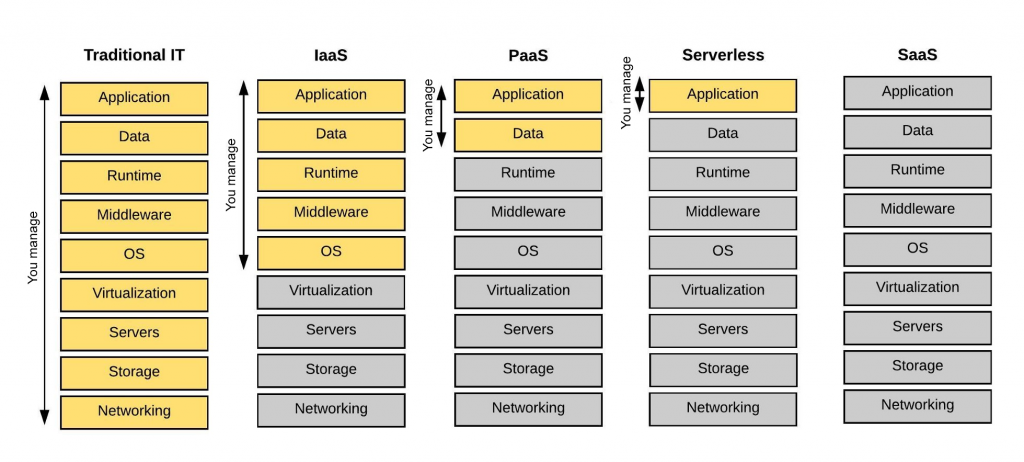
\includegraphics[height=7cm]{images/cloud-computing-service-models}
	\caption{مدل‌های رایانش ابری}
	\label{cloudComputingServiceModels}
\end{figure}

\newpage

\section{رایانش بدون سرور}

تعریف اصطلاح بدون سرور دشوار است، زیرا این اصطلاح گمراه کننده است و تعریف آن هم بر مفاهیم دیگر مانند بستر نرم افزاری به عنوان سرویس (\lr{PaaS}) و نرم افزار به عنوان سرویس (\lr{SaaS}) همپوشانی دارد. بدون سرور بین این دو مفهوم قرار دارد، جایی که توسعه دهنده کنترل برخی زیرساخت های ابر را از دست می‌دهد، اما همانطور که در شکل \ref{developerControlAndServerless} توضیح داده شده است، بر روی کد برنامه کنترل دارد. مفاهیم بدون سرور به دو دسته تقسیم می‌شوند:

\begin{figure}[!h]
	\centering
	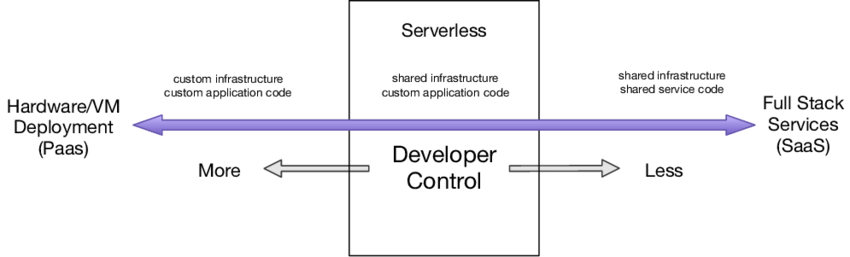
\includegraphics[height=4cm]{images/Developer-control-and-Serverless-computing}
	\caption{مقایسه میزان کنترل توسعه دهنده در مدل‌های رایانش ابری مختلف}
	\label{developerControlAndServerless}
\end{figure}

\subsection{\lr{Backend} به عنوان سرویس (\lr{BaaS})}

در مدل \lr{BaaS}\LTRfootnote{Backend as a Service} منطق سمت سرور توسط کاربر پیاده‌سازی و مدیریت نشده و در عوض از سرویس های ارائه دهنده استفاده می‌شود. این مدل بسیار نزدیک به مفهوم نرم افزار به عنوان سرویس (\lr{SaaS}) است تا سر و کار داشتن با ماشین های مجازی و کانتینرها. در این مدل، برنامه ها به اجزای کوچک تر تقسیم می‌شوند و تعدادی از این اجزاء کاملا با محصولات برون‌سپاری شده پیاده‌سازی می‌شوند.

سرویس های \lr{BaaS} دارای دامنه های عمومی‌هستند و از راه دور و از طریق \lr{API}\LTRfootnote{Application Programming Interface} مورد استفاده قرار می‌گیرند. این سرویس ها بیشتر مورد توجه توسعه دهندگان برنامه تلفن همراه و صفحات وب ثابت قرار گرفته است زیرا به راحتی می‌توانند برای انجام کارهای مورد نیازشان از این سرویس ها استفاده کنند. برای مثال \lr{Firebase} گوگل یک پایگاه داده است که کاملا توسط خود گوگل مدیریت می‌شود و از آن مستقیماً می‌توان در هر برنامه کاربردی و بدون نیاز به هیچ سروری استفاده کرد.

نمونه دیگر سرویس های \lr{BaaS} استفاده از منطق برنامه ای است که توسط تیم های دیگر پیاده‌سازی شده. به عنوان مثال سرویس هایی مانند \lr{Auth0} و \lr{Cognito} برای احراز هویت کاربران و مدیریت آن ها وجود دارند که برنامه های وب و تلفن همراه می‌توانند از آن استفاده کنند بدون این که نیاز داشته باشند تیم توسعه آن ها حتی قسمتی از این منطق را خودشان پیاده‌سازی کنند.

\lr{BaaS} به خاطر رشد در زمینه  توسعه برنامه های کاربردی تلفن همراه معروف شد و گاهی اوقات به \lr{MBaaS}\LTRfootnote{Mobile Backend as a Service} شناخته می‌شد. اما این مفهوم به \lr{backend} برای برنامه های کاربردی تحت وب و موبایل محدود نمی‌شود و به عنوان مثال می‌توان از سرویس هایی برای مدیریت سیستم فایل و ذخیره سازی داده و حتی آنالیز گفتار استفاده کرد که کاملا توسط شرکت دیگری ارائه و مدیریت می‌شوند. همچنین از این سرویس‌ها در سمت سرور نیز می‌توان بهره برد.

\subsection{تابع به عنوان سرویس (\lr{FaaS})}

در مدل سرویس دهی \lr{FaaS}\LTRfootnote{Function as a Service}، منطق سمت سرور همچنان توسط خود برنامه نویسان نوشته شده و کنترل می‌شود. اما برنامه ها در کانتینرهای فاقد وضعیت و گذرایی اجرا می‌شوند و که به وسیله رویدادها ایجاد شده اند.

تابع به عنوان سرویس در بسیاری از موارد برای تعریف کردن مفهوم بدون سرور استفاده می‌شود و بسیاری از افراد به اشتباه این دو مفهوم را به جای یکدیگر به کار می‌برند. \lr{FaaS} به نسبت بقیه مفاهیم بدون سرور جدیدتر است و برای پیاده‌سازی پروژه تمرکز ما بر روی این مدل سرویس بیشتر خواهد بود، بنابراین بیشتر به توضیح کارکرد آن خواهیم پرداخت.
هنگامی‌که می‌خواستیم برنامه سمت سرور را به روش های متداول قدیمی‌پیاده‌سازی کنیم، ابتدا با یک سرور میزبان، یک ماشین مجازی یا حتی یک کانتینر شروع به کار می‌کردیم. سپس برنامه خود را درون آن میزبان مستقر می‌کردیم. چنانچه میزبان یک ماشین مجازی یا کانتینر بود، برنامه ما به عنوان یک پردازه سیستم عامل اجرا می‌شد. معمولا برنامه ما متشکل بود از کدهایی که برای انجام عملیات های مختلف و مرتبط با هم نوشته شده بودند.

\lr{FaaS} این نوع پیاده‌سازی را تغییر داد. به این صورت که میزبان و پردازه‌ی برنامه از این مدل حذف شدند و تمرکز بر پیاده‌سازی منطق برنامه به صورت عملیات ها و تابع های جداگانه قرار گرفت. این تابع ها پس از توسعه به صورت جداگانه بر روی بستر ‌\lr{FaaS} قرار گرفته و اجرا می‌شوند. اما این تابع ها مانند یک پردازه‌ی سرور نیستند که  پیوسته فعال باشند و در وضعیت \lr{idle} قرار داشته باشند تا اینکه زمان اجرای آن‌ها برسد. در عوض بستر \lr{FaaS} طوری ساخته شده که برای هر تابع منتظر رویداد مربوط به آن بماند. زمانی که آن رویداد رخ داد، بستر از تابع مربوط به آن یک نمونه می‌سازد، سپس آن نمونه را با پارامترهای آن رویداد اجرا می‌کند. هنگامی که اجرای تابع به اتمام رسید، بستر \lr{FaaS} آزاد است که آن را حذف کند، اما ممکن است آن را برای بهینه سازی مدتی آن را نگه دارد تا اگر رویداد جدیدی رخ داد نخواهد آن را از ابتدا بسازد.

\lr{FaaS} یک رویکرد رویداد محور\LTRfootnote{event-driven} است که علاوه بر ارائه یک بستر برای میزبانی و اجرای توابع با بسیاری از منابع رویدادی همگام و ناهمگام ادغام شده است. برای مثال \lr{HTTP API Gateway} یک منبع رویداد همگام است و صف پیام، عملیات ذخیره‌سازی یا رویدادهای برنامه‌ریزی شده، از منابع رویداد ناهمگام هستند.

از نظر سطحی، \lr{BaaS} و \lr{FaaS} کاملاً متفاوت هستند. مورد اول برون‌سپاری کامل اجزای برنامه به صورت جداگانه است و مورد  دوم یک محیط میزبانی جدید برای اجرای کد شخصی افراد است. پس چرا آن ها با هم زیر مجموعه مفهوم بدون سرور قرار می‌گیرند؟

دلیل اصلی این است که در هر دو مورد توسعه دهنده نیاز نیست که مدیریت زیرساخت های سرور خودش و یا پردازه های سرور را در نظر بگیرد. بلکه تمامی منطق برنامه در یک محیط عملیاتی کاملاً منعطف اجرا می‌شود و وضعیت برنامه نیز در محیطی متشابه ذخیره می‌گردد. با تغییر تقاضا روی سرور، بستر بدون سرور بر این اساس تعداد ظرفیت سرورها را افزایش داده و یا کاهش می‌دهد، بدون اینکه لازم باشد برنامه نویسی توسط توسعه دهنده انجام شود. هزینه میزبانی یک سرویس بدون سرور معمولاً متناسب با تعداد درخواست های اجرای تابع ها محاسبه می‌شود. به عبارت دیگر بدون سرور به این معنی نیست که واقعا سروری در کار نباشد بلکه بدین معنی است که دیگر نیازی نیست نگران سرور باشید \cite{roberts_chapin_2017}.

\begin{figure}[!h]
	\centering
	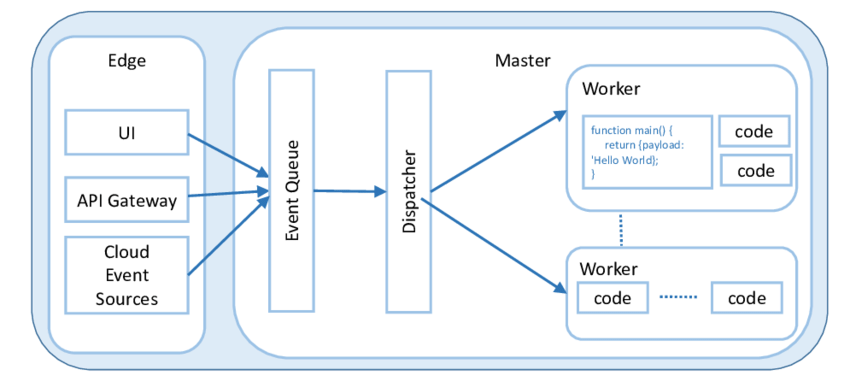
\includegraphics[height=7cm]{images/Serverless-platform-architecture}
	\caption{مثال ابتدایی از معماری یک بستر بدون سرور}
	\label{ServerlessPlatformArchitecture}
\end{figure}

مانند آنچه در شکل \ref{ServerlessPlatformArchitecture} مشاهده می‌شود، عملکرد اصلی بستر بدون سرور متکی است به توانایی پردازش رویدادها بر اساس تقاضا، با استفاده از مجموعه ای از توابع. بستر بدون سرور باید به مدیریت مجموعه‌ای از توابع، دریافت درخواست های \lr{HTTP} یا نوع دیگری از درخواست‌ها بپردازد، درخواست را با یکی از توابع مرتبط سازد، نمونه‌ای از تابع را ایجاد کند یا یک مورد موجود را پیدا کند و رویداد را به آن بفرستد، منتظر پاسخ از نمونه‌ی تابع باشد، با پاسخ از نمونه‌ی تابع به درخواست \lr{HTTP} پاسخ دهد و در صورت عدم نیاز نمونه‌ی تابع را خاموش کند. گزارش‌های مربوط به کل فرآیند را نیز باید هنگام انجام تمام این کارها جمع آوری کند. چالش اصلی بستر بدون سرور ارائه همه این موارد است در حالی که باید با الزاماتی از قبیل هزینه، تحمل خطا و مقیاس پذیری کنترل شود. چالش هایی که یک بستر بدون سرور باید بر آن غلبه کند، عبارتند از
\cite{pinto_dias_ferreira_2018}
\cite{baldini_2017}
:

\begin{itemize}
	
	\item سرعت برای شروع اجرای یک تابع و پردازش رویداد.
	
	\item صف رویدادها و سازگاری متناسب با آن ها. با توجه به ورود رویداد ها و وضعیت فعلی صف، باید برنامه زمانبندی اجرای تابع تنظیم و مدیریت شود تا منابع را از توابعی که در حال اجرا نیستند پس بگیرد.
	
	\item چگونگی مقیاس پذیری و مدیریت خطاها را با دقت در نظر بگیرد.
	
\end{itemize}

همانطور که در شکل مشاهده می‌شود، از زمان شکل گیری مفهوم بدون سرور، محبوبیت آن بسیار افزایش یافته است و انتظار می‌رود که این رشد همراه با رشد \lr{IoT} ادامه داشته باشد. رشد محبوبیت فناوری بدون سرور در شکل \ref{serverless_google_trends} قابل مشاهده است.

\begin{figure}[!h]
	\centering
	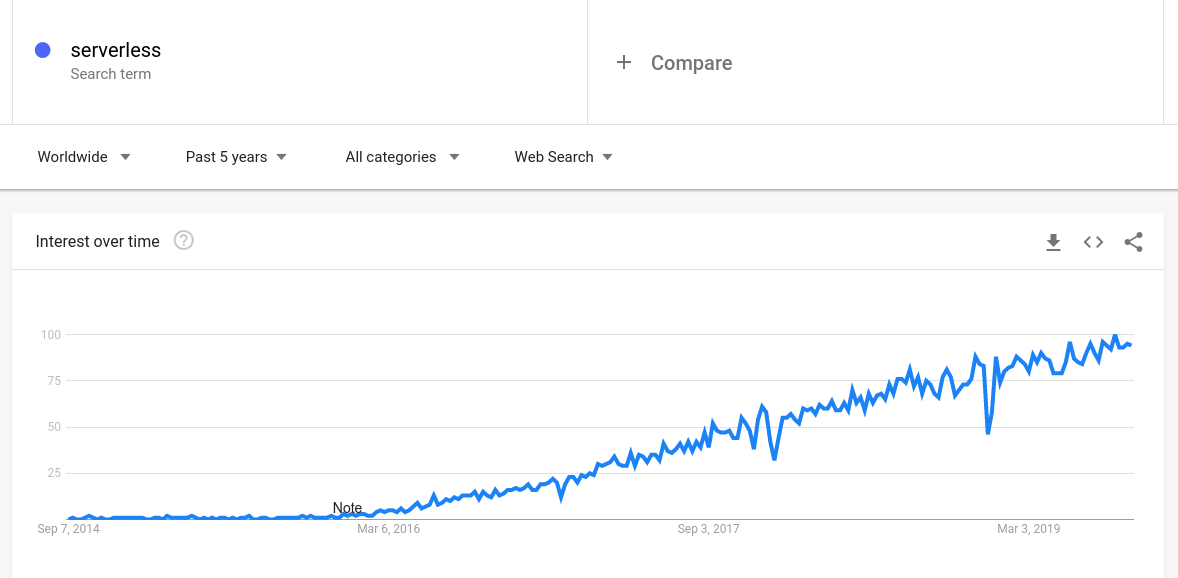
\includegraphics[height=8cm]{images/serverless_google_trends}
	\caption{افزایش محبوبیت کلمه \lr{serverless} ‌‌در \lr{‌Google Trends} طی سه سال اخیر}
	\label{serverless_google_trends}
\end{figure}

\subsection{راه حل‌ها و بسترهای ابری موجود}

\begin{itemize}
	
	\item \textbf{\lr{Amazon lambda}}  اولین بستری است که مدل سرویس بدون سرور را پیاده‌سازی کرد و معیارهای آن از جمله  قیمت گذاری، مدل برنامه نویسی، نحوه استقرار، محدودیت منابع، امنیت و مانیتورینگ را به بازار معرفی کرد. \lr{Lambda} از زبان های برنامه نویسی \lr{Node.js}، \lr{Python}، \lr{Java}  و \lr{C\#} پشتیبانی می‌کند. با توجه به این که این بستر در این زمینه پیشگام بوده است به عنوان اولین و بهترین راه حل انتخاب می‌شود و تعداد زیادی از شرکت های بزرگ از سرویس های این بستر استفاده می‌کنند.
	
	\item \textbf{\lr{Google Cloud Functions}}   در حال حاضر این بستر بسیار محدود است و تنها از زبان \lr{JavaScript} که در محیط استاندارد \lr{Node.js} نوشته شده باشد پشتیبانی می‌کند و تنها به رویدادهای سرویس \lr{Google Cloud} یا درخواست های \lr{HTTP} پاسخ می‌دهد. همچنین این بستر هنوز در فاز بتا است و نسخه نهایی آن منتشر نشده است.
	
	\item \textbf{\lr{Microsoft Azure Functions}}  بستر بدون سرور متن بازی را ارائه می‌دهد که کد آن در \lr{Github} موجود است. تابع های ارائه شده توسط توسعه دهنده با \lr{HTTP webhook} که با سرویس های بستر ادغام شده است اجرا می‌شوند. این بستر نیز از زبان های محدودی پشتیبانی می‌کند.
	
	\item \textbf{\lr{OpenLambda}}  بستر بدون سرور و متن باز جدیدی است که کد آن در \lr{Github} موجود است. این بستر در مواردی مشکل دارد که توسعه دهندگان در حال رفع آن هستند \cite{openlambda}:
	
	\begin{enumerate}

		\item راه اندازی بسیار آهسته \lr{runtime} های زبان‌های برنامه نویسی
		
		\item استقرار حجم زیادی از کد
		
		\item پشتیبانی از حفظ وضعیت که با تابع های فاقد وضعیت پیاده شده باشد

		\item استفاده از پایگاه داده‌ها

	\end{enumerate}

	\item \textbf{\lr{Kubeless}} این بستر بدون سرور، با راه‌اندازی بر روی بستر کوبرنتیز، بدون نیاز به پیچیدگی‌های چارچوب بستر بدون سرور مانند سیستم صف پیام، آن را به یک بستر اجرا کننده‌ی تابع تبدیل می‌کند. اما این بستر هنوز به اندازه کافی بالغ نشده است که در مرحله تولید مورد استفاده قرار گیرد. همچنین جامعه‌ی آن به اندازه کافی بزرگ نیست، اسناد آن ناقص هستند و اشکالاتی در آن مشاهده شده است. این بستر نیز متن باز است \cite{kubeless}.
	
	\item \textbf{\lr{OpenFaaS}} یکی از بهترین و معروف‌ترین بستر بدون سرور متن باز با استفاده‌ی آسان است. تابع‌ها در بستر \lr{OpenFaaS} باید از جنس کانتینر باشند. به همین دلیل این بستر از تمامی زبان‌های برنامه نویسی پشتیبانی می‌کند. معماری این بستر نسبتاً ساده است و بر روی هماهنگ کننده‌های ابری کوبرنتیز و \lr{Docker Swarm} راه‌اندازی می‌شود \cite{openfaas}.
	
	\item \textbf{\lr{OpenWhisk}}  کلیدی ترین ویژگی این بستر این است که می‌توان با اتصال تابع ها با یکدیگر ترکیبی از تابع ها را ساخت و آن را به عنوان تابع جدید ارائه داد. این بستر نیز به صورت متن باز در \lr{Github} موجود است و از زبان های \lr{Node.js}، \lr{Java}، \lr{Swift} و \lr{Python} پشتیبانی می‌کند. همچنین این قابلیت نیز وجود دارد که تابع ها به صورت باینری پیاده‌سازی شده و در یک کانتینر قرار گرفته باشند.
	
	این بستر در مقایسه با معماری ساده بدون سرور (شکل \ref{ServerlessPlatformArchitecture})، دارای اجزای مهمی است که امنیت، گزارش گرفتن و نظارت را کنترل می‌کنند. این معماری جدید در شکل \ref{OpenWhisk-architecture} قابل مشاهده است.
	
	\begin{figure}[!h]
		\centering
		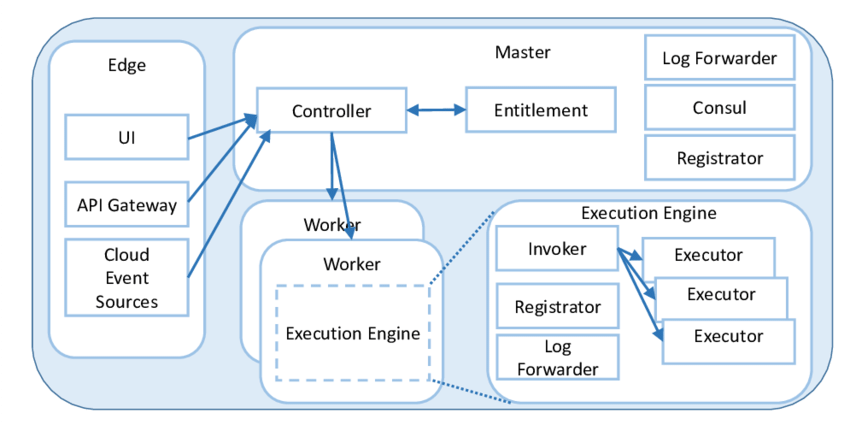
\includegraphics[height=7cm]{images/OpenWhisk-architecture}
		\caption{معماری بستر بدون سرور \lr{OpenWhisk}}
		\label{OpenWhisk-architecture}
	\end{figure}
	
\end{itemize}

در انتها به این نتیجه می‌رسیم که بهترین و پایدارترین راه حل \lr{AWS Lambda} است. پیشگام بودن در این زمینه باعث شده است تا وقت کافی برای رشد و پشتیبانی از زبان های معروف را داشته باشد. بعد از آن \lr{Microsoft Azure Functions} برای انتخاب مناسب است. به دلیل در دسترس نبودن این سرویس‌ها در داخل کشور، پیاده‌سازی این بستر با بهره گیری از پروژه های متن باز معقول به نظر می‌رسد و ارائه چنين سرويس‌هايي در حال آغاز است. با توجه به بررسی‌ها و مقایسه‌های صورت گرفته بهترین راه حل متن باز استفاده از بستر \lr{OpenWhisk} است که ما در این پروژه نیز از این بستر استفاده کردیم. در ادامه پس از آشنایی با مفاهیم و معماری میکروسرویس، بیشتر با نحوه کارکرد و اجزای مختلف این بستر بدون سرور آشنا خواهیم شد.

\newpage

\section{میکروسرویس و کانتینرها}

معماری میکروسرویس\LTRfootnote{microservices architectur} به مرور در حال کسب محبوبیت فزاینده‌ای است و امروزه تقریباً در همه پروژه‌های نرم‌افزاری عمده از آن استفاده می‌شود. دلیل اصلی این مسئله ناشی از مزیت‌های آن و مسائلی است که حل می‌کند. در این بخش ابتدا به معرفی مفهوم معماری میکروسرویس و شناخت مزیت‌های استفاده از آن می‌پردازیم و سپس فناوری‌های مورد نیاز برای پیاده‌سازی این نوع معماری را بررسی می‌کنیم.

\subsection{میکروسرویس}

در ابتدا باید مفهوم خود میکروسرویس را درک کنیم. میکروسرویس، همان طور که از نام آن مشخص می‌شود، اساساً به سرویس‌های نرم‌افزاری مستقلی گفته می‌شود که کارکردهای تجاری خاصی را در یک برنامه‌ی کاربردی نرم‌افزاری ارائه می‌کنند. این سرویس‌ها می‌توانند به صورت مستقل از هم نگهداری، نظارت و توزیع شوند.

معماری مبتنی بر سرویس\LTRfootnote{Services Oriented Architecture (SOA)} به برنامه‌های کاربردی‌ امکان ارتباط با یکدیگر روی یک رایانه منفرد و یا در زمان توزیع برنامه‌های کاربردی‌ روی چندین رایانه در یک شبکه را ارائه می‌کند. هر میکروسرویس ارتباط اندکی با سرویس‌های دیگر دارد. این سرویس‌ها خودکفا هستند و یک کارکرد منفرد (یا گروهی از کارکردهای مشترک) را ارائه می‌کنند.

معماری میکروسرویس‌ها به طور طبیعی در سازمان‌های بزرگ و پیچیده استفاده می‌شود که در آن‌ها چند تیم توسعه می‌توانند مستقل از هم برای ارائه یک کارکرد تجاری کار بکنند و یا برنامه‌های کاربردی‌ ملزم به ارائه خدمات به یک حوزه تجاری باشند.

به طور خلاصه یک مفهوم وجود دارد و آن این است که ما همواره ملزم هستیم نرم‌افزار را نگهداری و به‌روزرسانی کنیم. باید فرایند بهبود برنامه‌های کاربردی‌ را آسان‌تر و مقدار زمان مورد نیاز برای ارائه نسخه‌های جدید آن‌ها را کوتاه‌تر کنیم.

\subsubsection{معماری یکپارچه}

در سال‌های اخیر برنامه‌های کاربردی‌ نرم‌افزاری در معماری‌های چندلایه و یکپارچه پیاده‌سازی می‌شدند. به عنوان نمونه در شکل \ref{monolithic} یک معماری معمول برای برنامه‌ی کاربردی یکپارچه ارائه شده است:

\begin{figure}[!h]
	\centering
	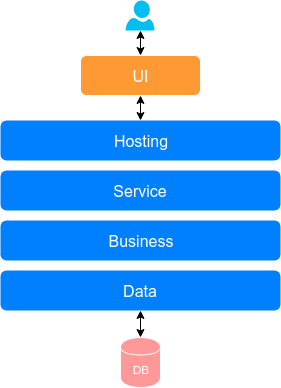
\includegraphics[height=8cm]{images/monolithic-architecture}
	\caption{معماری یکپارچه}
	\label{monolithic}
\end{figure}

در این معماری هر لایه در کد نرم‌افزاری پیاده‌سازی می‌شد و از چندین کلاس و واسط تشکیل شده بود:

\textbf{لایه داده}

این لایه برای ذخیره‌سازی داده‌ها در پایگاه داده و فایل‌ها پیاده‌سازی شده است. تنها مسئولیت این لایه ارائه داده‌ها از منابع داده‌ای مختلف است.

\textbf{لایه تجاری}

مسئولیت لایه تجاری، بازیابی داده‌ها از لایه داده و اجرای محاسبات است. لایه تجاری نمی‌داند که داده‌ها در فایل یا پایگاه داده یا در موارد دیگر هستند. لایه تجاری به لایه داده‌ها وابسته است.

\textbf{لایه سرویس}

لایه سرویس روی لایه تجاری قرار می‌گیرد. این لایه یک پوشش برای لایه تجاری ایجاد می‌کند که شامل امنیت، گزارش‌گیری و وساطت برای فراخوانی کارکردها است. لایه سرویس به لایه تجاری وابسته است.

\textbf{لایه میزبانی}

سرویس‌ها از طریق این لایه میزبانی می‌شوند. لایه میزبانی از فناوری‌های مبتنی بر سرویس مانند \lr{REST API} برای میزبانی با استفاده از پروتکل‌های مختلف مانند \lr{HTTP} ،\lr{HTTPS} ،\lr{TCP} و غیره بهره می‌گیرد. کل برنامه‌ی کاربردی به صورت یک پردازش نرم‌افزاری اجرا می‌شود. برنامه‌‌ها از طریق \lr{URL} مانند \lr{https://example.com/myapplication} در دسترس هستند.

\textbf{لایه رابط کاربری}

لایه رابط کاربری شامل کدهایی است که در لایه میزبانی مورد ارجاع قرار می‌گیرند و به منظور ایجاد امکان تعامل با برنامه‌ی کاربردی برای کاربران طراحی شده است.

این طراحی به توسعه‌دهندگان امکان می‌دهد که روی یک کارکرد خاص متمرکز شوند، ویژگی را تست کنند، و یا برنامه‌ی کاربردی را با استفاده از کنترل معکوس از طریق تزریق وابستگی‌ها و میزبانی یک برنامه‌ی کاربردی روی ماشین‌های متعدد تجزیه کنند.

طراحی یکپارچه لایه‌بندی شده مزایای زیادی دارد؛ اما نواقصی نیز دارد. در ادامه فهرستی از مشکلات رایج این نوع معماری را مورد اشاره قرار داده‌ایم:

\begin{itemize}
	
	\item این طراحی برای مقیاس‌بندی و نگهداری برنامه‌ی کاربردی سرراست نیست. این طراحی زمان مورد نیاز برای قرار دادن کارکردهای جدید در اختیار کاربر را افزایش داده است، چون چرخه توسعه زمان بیشتری طول می‌کشد.
	
	\item از آنجا که کل برنامه‌ی کاربردی به صورت یک پردازش منفرد میزبانی می‌شود، هر بار که لازم باشد یک به‌روزرسانی اجرا شود، کل برنامه‌ی کاربردی باید متوقف شود و سپس نسخه جدیدی از آن باید توزیع شود.
	
	\item برای ایجاد تعادل در بار کاری، کل برنامه‌ی کاربردی روی چند ماشین توزیع می‌شود. به علاوه، امکان توزیع کارکردهای خاص روی سرورهای چندگانه برای متوازن‌سازی بار وجود ندارد.
	
	\item طراحی برنامه‌ی کاربردی پیچیده است، چون همه ویژگی‌ها در یک برنامه‌ی یکپارچه منفرد پیاده‌سازی شده‌اند.
	
	\item زمانی که تعداد برنامه‌های کاربردی‌ در سازمان افزایش می‌یابد، توزیع برنامه‌های یکپارچه نیازمند اطلاع‌رسانی و هماهنگی با همه تیم‌های توسعه ویژگی‌های جدید است. این امر موجب افزایش زمان مورد نیاز برای تست و توزیع برنامه می‌شود.
	
	\item این معماری برنامه‌ی کاربردی را وادار می‌کند که در یک مجموعه فناوری منفرد پیاده‌سازی شود.
	
	\item در مواردی که زمان تحویل طولانی‌تر شود، در طی زمان نیازمند پول بیشتری برای توسعه و نگهداری برنامه‌ی کاربردی خواهد بود.
	
	\item از آنجا که همه کد درون یک برنامه‌ی کاربردی منفرد قرار دارد، نگهداری کد پس از مدتی به سرعت دشوار می‌شود.
	
\end{itemize}

\subsubsection{معماری میکروسرویس}

میکروسرویس‌ها برای حل مسائل اشاره شده فوق معرفی شده‌اند. معماری میکروسرویس یک بهینه‌سازی در زمینه معماری یکپارچه محسوب می‌شود. در این معماری هر کارکرد تجاری به صورت یک سرویس ارائه می‌شود. هر سرویس می‌تواند به صورت مستقل از سرویس‌های دیگر میزبانی و توزیع شود. در شکل \ref{microservices} معماری یکپارچه با معماری میکروسرویس مقایسه شده است.

\begin{figure}[!h]
	\centering
	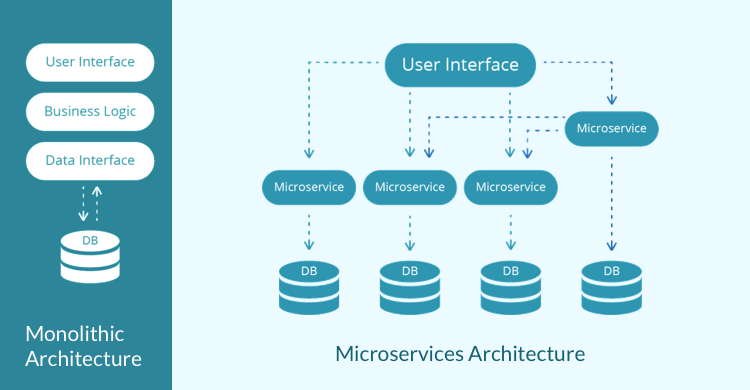
\includegraphics[height=8cm]{images/monolithic-vs-microservices}
	\caption{مقایسه معماری میکروسرویس با معماری یکپارچه}
	\label{microservices}
\end{figure}

\begin{itemize}
	
	\item هر سرویس را می‌توان یک برنامه‌ی کاربردی کوچک تصور کرد.
	
	\item همه سرویس‌ها می‌توانند حتی زمانی که سرویس‌ها روی ماشین‌های مختلف هستند، با همدیگر ارتباط داشته باشند. این وضعیت در ادامه امکان پیاده‌سازی کارکردهای جدید در سرویس‌ها را فراهم می‌سازد.
	
	\item میکروسرویس‌ها، سازمان‌ها را تشویق می‌کنند که از فرایند توزیع و تحویل پیوسته\LTRfootnote{Continuous Integration/ Continuous Development (CI/CD)} خودکار پیروی کنند.
	
	\item برنامه‌های کاربردی‌ در نهایت بسیار پایدارتر می‌شوند، چون هر ویژگی می‌تواند به صورت مستقل تست و توزیع شود.
	
	\item از آنجا که هر سرویس روی پردازش مجزایی میزبانی می‌شود، اگر یک سرویس به نقطه تنگنای برنامه‌ی کاربردی تبدیل شود و به منابع زیادی نیاز داشته باشد، در این صورت می‌توان آن را بدون هیچ گونه تأثیر سوء روی سرویس‌های دیگر، به ماشین دیگری انتقال داد.
	
	\item زمانی که کاربران بیشتری شروع به استفاده از یک ویژگی برنامه‌ی کاربردی بکنند، آن سرویس می‌تواند با توزیع روی رایانه‌های قدرتمندتر یا از طریق استفاده از کش بدون این که روی سرویس‌های دیگر هیچ تأثیری بگذارد، مقیاس‌بندی شود.
	
	\item این معماری پایداری برنامه‌ی کاربردی را نیز افزایش می‌دهد، چون هر سرویس می‌تواند به صورت مستقل ساخته، تست، توزیع و استفاده شود.
	
	\item کد برنامه‌ی کاربردی می‌تواند به سادگی نگهداری شود و پردازش‌ها می‌توانند به صورت مجزا تحت نظارت قرار بگیرند.
	
	\item توسعه‌دهندگان اختصاصی می‌توانند سرویس‌ها را به صورت مستقل از هم پیاده‌سازی کرده و این سرویس‌ها را بدون تأثیرگذاری روی سرویس‌های دیگر انتشار دهند.
	
	\item بدین ترتیب نقطه شکست منفرد نیز از بین می‌رود، زیرا یک سرویس می‌تواند بدون تأثیرگذاری روی ویژگی‌های دیگری که برنامه‌ی کاربردی نرم‌افزاری ارائه می‌کند، متوقف شود.
	
	\item در نتیجه این طراحی زمان مورد نیاز برای تحویل نسخه‌های جدید را کاهش می‌دهد و بنابراین هزینه را در طی زمان کاهش می‌دهد.
	
	\item قابلیت استفاده مجدد از کد افزایش می‌یابد، زیرا یک ویژگی به صورت سرویس میزبانی شده است و امکان استفاده چند سرویس از یک ویژگی به جای پیاده‌سازی مجدد کد در هر مورد وجود دارد.
	
	\item معماری مبتنی بر سرویس امکان استفاده از مجموعه متنوعی از فناوری‌ها برای رفع نیازها را دارد. به عنوان نمونه بسته‌های تحلیل داده زبان پایتون می‌توانند به صورت مجزا توزیع و میزبانی شوند و همزمان می‌توان از \lr{NodeJS} برای پیاده‌سازی سرویس‌ها استفاده کرد و \lr{ReactJS} نیز برای پیاده‌سازی رابط کاربری مورد استفاده قرار گیرد.
	
\end{itemize}

در شکل \ref{distribution-microservices} نشان داده‌ایم که سرویس‌های متفاوت چگونه می‌توانند روی سرورهای مختلف برنامه‌ی کاربردی توزیع شوند \cite{malik_2019}.

\begin{figure}[!h]
	\centering
	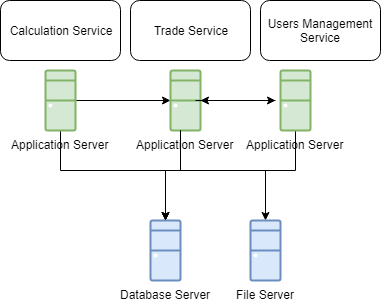
\includegraphics[height=7cm]{images/distribution-microservices}
	\caption{توزیع میکروسرویس‌ها روی سرورهای مختلف}
	\label{distribution-microservices}
\end{figure}

میکروسرویس‌ها می‌توانند با استفاده از طیف متنوعی از فناوری‌ها از جمله داکر و کوبرنتیز پیاده‌سازی و میزبانی شوند. در ادامه به معرفی این فناوری‌ها می‌پردازیم. اما در ابتدا نیاز به آشنایی با مفهوم کانتینر\LTRfootnote{container} داریم.

\subsection{کانتینرها}

کانتینرها اجازه بسته‌بندی برنامه‌های کاربردی را به همراه تمام قسمت‌هایی که نیاز دارند شامل کتابخانه‌ها و دیگر وابستگی‌هایش، به توسعه‌دهنده‌ها می‌دهند. به عبارت دیگر می‌توانیم کانتینر را شامل پردازه\LTRfootnote{process} در حال اجرا و منابع سخت‌افزاری اختصاص داده شده به آن پردازه تعریف کرد (شکل \ref{container}). پس کانتینر به معنی یک قسمت سخت‌افزاری و قابل رویت نیست بلکه یک تعریف انتزاعی به معنای یک پردازه یا گروهی از پردازه‌ها به همراه منابع تخصیص داده شده به آن‌ها می‌باشد. 

\begin{figure}[!h]
	\centering
	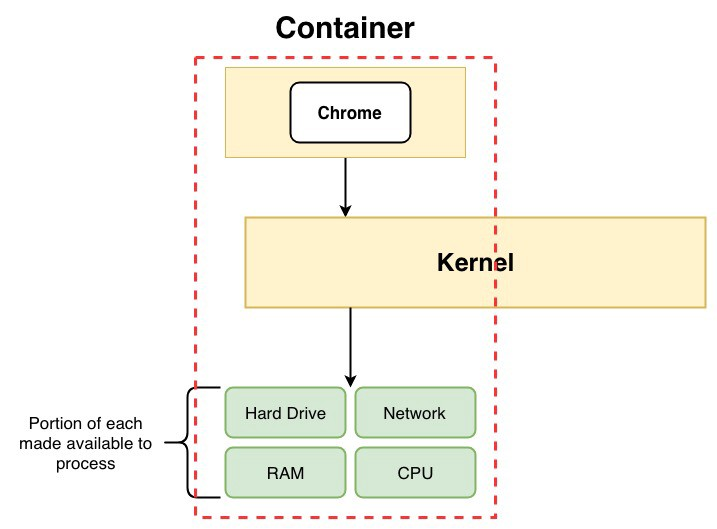
\includegraphics[height=7cm]{images/container}
	\caption{نمایش یک کانتینر}
	\label{container}
\end{figure}

کانتینرها مکانیزم منطقی بسته‌بندی ارائه می‌دهند بدین معنا که برنامه‌های کاربردی می‌توانند از محیطی که در آن در حال اجرا هستند جدا شوند. این جداسازی باعث می‌شود تا برنامه‌های کاربردی مبتنی بر کانتینرها به راحتی و بدون درنظر گرفتن محیط هدف مستقر شوند. کانتینرایز کردن برنامه‌ها منجربه آن می‌شود که توسعه‌دهندگان تنها به منطق برنامه فکر کنند و تیم‌های عملیات تکنولوژی اطلاعات بر روی پیاده‌سازی و مدیریت آن تمرکز کنند.

برخلاف یک ماشین مجازی، یک کانتینر دارای یک سیستم عامل مجزا نمی‌باشد. سیستم عامل‌ها
\lr{kernel}
دارند که یک پروسه اجرایی نرم‌افزاری\LTRfootnote{running software process} می‌باشد و وظیفه آن کنترل دسترسی بین برنامه‌های در حال اجرا به منابع سخت‌افزاری موجود در کامپیوتر است.

سیستم عامل‌ها ویژگی به نام
\lr{name spacing}
دارند که به وسیله آن می‌شود قطعه‌هایی\LTRfootnote{segments} از منابع سخت‌افزاری موجود ساخت و آنها را به یک برنامه خاص اختصاص داد. در نتیجه به وسیله
\lr{name spacing}
می‌شود منبع سخت‌افزاری را بر طبق  پردازه یا برنامه اجرایی جدا و ایزوله کرد. البته ویژگی
\lr{name spacing}
فقط برای سخت‌افزار نمی‌باشد و برای نرم‌افزار هم تعریف می‌شود. یک ویژگی دیگر هم با نام
\lr{control group}
وجود دارد که به وسیله آن می‌توان مقدار منبعی که یک پردازه می‌تواند استفاده کند را محدود کرد. در نتیجه به وسیله این دو ویژگی می‌توان برای هر پردازه منابعی را اختصاص داد و آن منابع را محدود کرد. 

در این میان نیاز به تعریف مفهومی با عنوان ایمیج\LTRfootnote{image}داریم. ایمیج فایل‌های سیستمی\LTRfootnote{file system} است که شامل همه‌ی وابستگی‌ها و تنظیمات موردنیاز برای اجرای یک برنامه خاص می‌باشد. ایمیج را می‌توان به کانتینر تبدیل کرد. برای این کار ابتدا
\lr{kernel}
منابع سخت‌افزاری لازم را جدا می‌کند به طوری که فقط پردازه‌های کانتینر موردنظر می‌توانند به این منابع دسترسی داشته باشند. در ادامه فایل‌های موردنیاز آن کانتینر نیز جدا می‌شوند و بدین ترتیب یک کانتینر ساخته می‌شود.


\subsection{داکر}

در قسمت قبل با مفهوم کانتینر آشنا شدیم. حال سوال این است که چگونه می‌توانیم کانتینر را بسازیم و سپس با آن کار کنیم؟ در این قسمت با ابزاری به نام داکر\LTRfootnote{Docker} آشنا می‌شویم.

داکر وظیفه مدیریت کانتینرها را به عهده دارد و بیشتر شبیه یک ماشین مجازی عمل می‌کند، تفاوت داکر با ماشین مجازی در این است که در ماشین مجازی برای اجرای برنامه‌ی کاربردی و برنامه های مختلف که بخواهیم به صورت ایزوله و مجزا از هم کار کنند باید ماشین‌های مجازی مختلف ساخته شود که همین موضوع بار پردازشی و هدر رفت منابع سیستمی را روی سرور به همراه دارد. ولی در داکر روی یک ماشین مجازی خاص که می‌تواند دارای سیستم عامل ویندوز یا لینوکس باشد، ماژول داکر نصب شده و سپس روی سرویس داکر، کانتینرهای مختلف حاوی برنامه‌های کاربردی مختلف نصب و اجرا می‌شوند بدون اینکه کانتینرها به هم دسترسی داشته باشند. (شکل \ref{dockerVsVm}) بدین صورت کانتینرها از هم ایزوله هستند و نیاز برای ایجاد چندین ماشین مجازی را مرتفع می‌سازند. از طرف دیگر کانتینرهای داکر به راحتی در فضای رایانش ابری قرار می‌گیرد و به نوعی طراحی شده که تقریباً تمامی برنامه‌های کاربردی که از متدولوژی توسعه عملیات\footnote{توسعه عملیات (\lr{DevOps})، مجموعه‌ای از روشها، فرایندها و ابزارهایی است که با تمرکز بر همکاری و یکپارچگی بین تیم‌های توسعه نرم‌افزار و عملیات فناوری اطلاعات، ارزش‌های تولید شده را به‌طور سریع و مداوم به مشتریان نهایی می‌رساند.} بهره می‌گیرند با داکر تعامل داشته باشند.

\begin{figure}[!h]
	\centering
	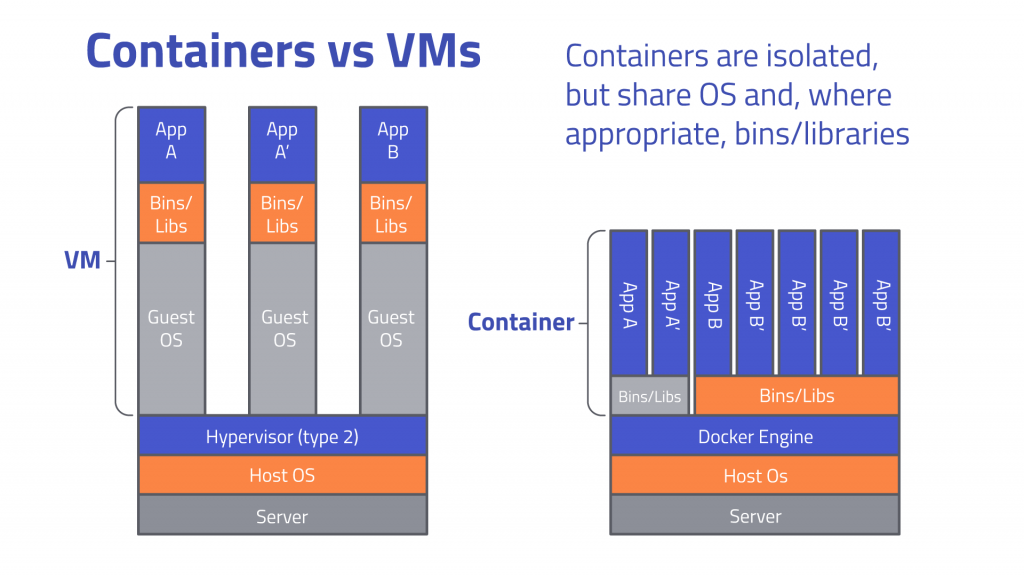
\includegraphics[height=9cm]{images/Docker-vs-VM}
	\caption{مقایسه‌ی داکر و ماشین مجازی}
	\label{dockerVsVm}
\end{figure}

داکر محیطی محلی را برای توسعه فراهم می‌کند که این محیط دقیقاً عمل‌کرد یک سرور را در اختیار توسعه‌دهندگان قرار می‌دهد. این امر برای روش توسعه توزیع و تحویل پیوسته (\lr{CI/CD}) کاربرد زیادی دارد. از این طریق می‌توان چندین محیط توسعه را از یک میزبان مشخص با یک نرم‌افزار، سیستم‌عامل و تنظیمات واحد اجرا کرد. از طرف دیگر پروژه‌ را می‌توان روی چند سرور جدید و مختلف آزمایش کرد و تمامی اعضای گروه بر روی یک پروژه‌ واحد با تنظیمات همانند قادر به همکاری هستند. این کار توسعه‌دهندگان را قادر می‌سازد تا نسخه‌های جدید برنامه خود را به سرعت آزمایش کرده و از عملکرد صحیح آن اطمینان خاطر حاصل کنند.

تمامی زیرساخت‌های فناوری اطلاعات نیازمند مدیریت و نظارت هستند و در همین راستا کانتینرها نیز باید نظارت شوند و در حالت کنترل‌شده‌ای قرار بگیرند. درغیر این‌ صورت مشخص نخواهد شد سرور چه برنامه‌هایی را اجرا می‌کند. خوشبختانه از برنامه‌های دواپس می‌توان برای مانیتور کانتینرهای داکر کمک گرفت، اما به این نکته نیز باید اشاره کرد که این برنامه‌ها برای کانتینرها بهینه‌ نشده‌اند. اینجاست که باید سراغ ابزارهای مدیریت و نظارت رایانش ابری را گرفت. ابزارهایی مانند \lr{Docker Swarm}, \lr{Kubernetes} و \lr{Mesosphere} در این زمینه گزینه‌های خوبی به‌نظر می‌رسند و تجربه نشان داده است در بین این ابزارها \lr{Kubernetes} محبوبیت بیشتری پیدا کرده است.
\cite{nichols_2018}

\subsection{کوبرنتیز}

\subsubsection{مفاهیم اولیه}

کوبرنتیز یک هماهنگ‌کننده‌ی کانتینری\LTRfootnote{container orchestration} متن باز، قابل حمل و قابل توسعه می‌باشد که برای اجرا و مدیریت کانتینرها و همچنین جهت تسهیل تنظیمات توسعه داده شده‌است. کوبرنتیز بر مبنای 15 سال تجربه گوگل در ساختن کانتینرها بنا شده‌است.

از ویژگی‌های کوبرنتیز می‌توان به موارد زیر اشاره کرد:
\begin{enumerate}
	\item 
	کشف سرویس و توزیع‌بار\LTRfootnote{Service discovery and load balancing}:\\
	کوبرنتیز بدون احتیاج به تغییر برنامه کاربردی این امکان را می‌دهد تا سرویس خود را ثبت نام کنید و اجازه دهید تا بقیه سرویس‌ها از وجود آن خبردار شوند. کوبرنتیز به هر کانتینر یک آدرس آی‌پی اختصاصی می‌دهد و برای هر گروه از کانتینرها یک نام \lr{DNS} اختصاص می‌دهد که امکان توزیع بار بین آن‌ها را فراهم می‌کند.
	\item 
	هدایت‌کردن انبارهای ذخیره اطلاعات\LTRfootnote{Storage orchestration}:\\
	کوبرنتیز این اجازه را می‌دهد تا به صورت خودکار انبارهای ذخیره اطلاعات سیستم را مقداردهی کنید.
	\item 
	تطبیق خودکار\LTRfootnote{Automated rollouts and rollbacks}:\\
	بدین معنی که حالت مورد انتظار خود را به کوبرنتیز معرفی می‌کنید و کوبرنتیز حالت فعلی را به حالت مورد انتظار تبدیل می‌کند.
	
	\item
	بسته‌بندی خودکار\LTRfootnote{Automatic bin packing}:\\
	با توجه به نیازمندی و منابع مورد‌نیاز هر کانتینر، کوبرنتیز به صورت اتوماتیک کانتینرها را بر روی نود‌ها قرار می‌دهد.
	\item
	ترمیم خودکار\LTRfootnote{Self-healing}:\\
	کوبرنتیز به صورت خودکار تمامی کانتینرهایی که موفق به اجرا نشوند را بازنشانی می‌کند. همچنین در صورتی که نودی که کانتینر بر روی آن در حال اجرا است، دچار مشکل شود، کوبرنتیز تمامی کانتینرهای در حال اجرا بر روی آن را مجدداً روی نود‌های باقی‌مانده قرار می‌دهد.
	\item
	توسعه‌پذیری افقی:\\
	کوبرنتیز این امکان را می‌دهد تا برنامه کاربردی خود را به صورت اتوماتیک کوچک یا بزرگ کنید. همچنین این امکان را می‌دهد تا این کار را بر عهده‌ی خود کوبرنتیز قرار دهید و این کار به صورت خودکار انجام گیرد.
	
	\item
	مدیریت 
	\lr{secret}
	ها و تنظیمات\LTRfootnote{Secret and configuration management}:\\
	کوبرنتیز امکان ذخیره و مدیریت اطلاعات حساس مانند رمز‌عبورها، 
	\lr{OAuth tokens}
	, 
	\lr{ssh keys}
	را می‌دهد. می‌توانید بدون بازسازی کانتینرها، 
	\lr{secrets}
	و تنظیمات، محصول کاربردی را پیاده‌سازی و یا به‌روز کنید. این کار بدون نمایش‌دادن 
	\lr{secret}
	در فایل‌های تنظیمات انجام می‌گیرد.
	
\end{enumerate}

\newpage

\subsubsection{معماری کوبرنتیز}
اولین مرحله جهت کار کردن با کوبرنتیز شناخت معماری و اجزای آن است.

یک نود کوچک‌ترین جزء سخت‌افزارهای محاسباتی در کوبرنتیز است. نود نماینده یک ماشین در خوشه است. در بیشتر سیستم‌های تولید، به احتمال زیاد نود یک ماشین فیزیکی در مرکز داده و یا یک ماشین مجازی بر روی ارائه‌دهندگان ابری می‌باشد. تعریف یک نود به عنوان یک ماشین، ‌این اجازه را می‌دهد که یک لایه از مفاهیم را استفاده  کنیم. بدین معنا که نیاز نیست نگران مشخصات یکتا ماشین باشیم بلکه هر ماشین را مجموعه‌ای منابع مانند \lr{CPU} و \lr{GPU} درنظر می‌گیریم که می‌توانند استفاده شوند. بدین ترتیب هر ماشین می‌تواند جایگزین ماشینی دیگر در دنیای کوبرنتیز شود.

اگرچه کارکردن با تک‌نودها می‌تواند مفید باشد اما این روش کوبرنتیز نیست. به طور کلی در کوبرنتیز ما یک خوشه\LTRfootnote{cluster} را به جای حالت‌های تک‌نودها درنظر می‌گیریم (شکل \ref{تصویر 2-9}). در کوبرنتیز نودها منابع خود را به اشتراک می‌گذارند تا یک ماشین قدرتمند‌تر شکل گیرد. وقتی برنامه‌های خود را بر روی خوشه مستقر می‌کنید، کارهای اجرایی برنامه به صورت هوشمندانه بر روی تک نودها توزیع می‌شود. اگر نودی اضافه یا حذف شود، خوشه کارها را بر روی نودها  جابه‌جا می‌کند. لازم به ذکر است برنامه و برنامه‌نویس با نحوه اجرای برنامه و توزیع آن بر روی نودها درگیر نیست.

\begin{figure}[!h]
	\centering
	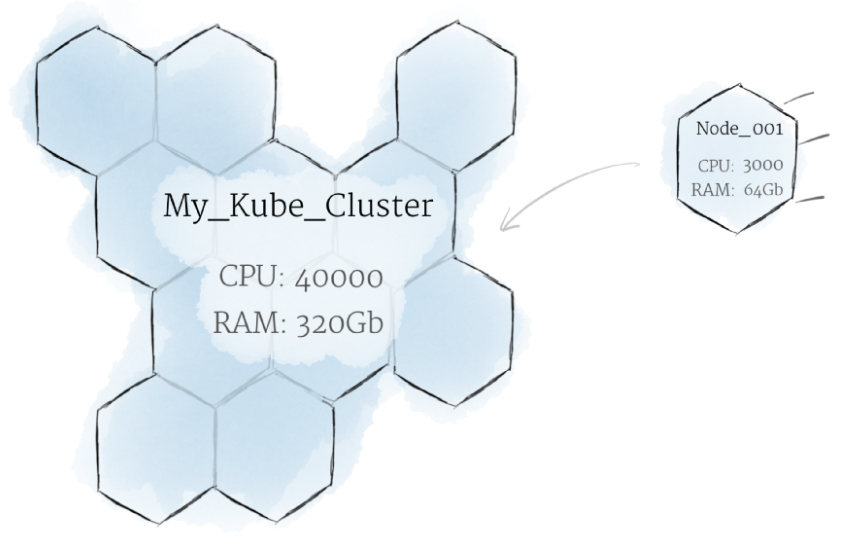
\includegraphics[height=7cm]{images/cluster-and-node}
	\caption{رابطه‌ی نود و خوشه در کوبرنتیز}
	\label{تصویر 2-9}
\end{figure}

تصویر (شکل \ref{تصویر 2-10}) معماری یک خوشه کوبرنتیز\LTRfootnote{Kubernetes Cluster}می‌باشد. از آن جایی که کوبرنتیز یک خوشه محاسباتی را پیاده می‌کند، همه چیز در داخل این خوشه کوبرنتیز اتفاق می‌افتد. این خوشه میزبانی یک نود با نام مستر\LTRfootnote{master} و نودهای دیگر با نام نود کارگر\LTRfootnote{worker node} را بر عهده دارد. همچنین خارج خوشه یک متعادل‌کننده بار\LTRfootnote{load balancer} وجود دارد که ترافیک خارجی را کنترل و بین نودها پخش می‌کند.  مستر کنترل خوشه و نودهای داخل آن را برعهده دارد. هر نود میزبان یک یا تعدادی پاد\LTRfootnote{pod} می‌باشد و هر پاد شامل گروهی از کانتیرها می‌باشد که برای یک هدف با یکدیگر در تعامل هستند.

\begin{figure}[!h]
	\centering
	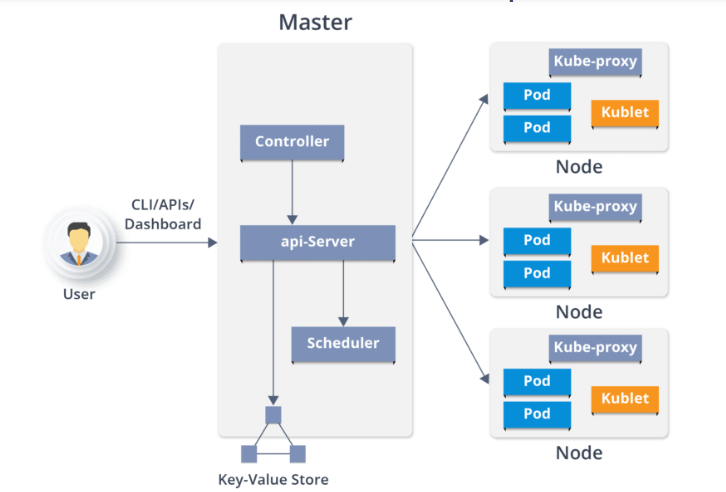
\includegraphics[height=8cm]{images/kubernetes-cluster}
	\caption{معماری خوشه کوبرنتیز}
	\label{تصویر 2-10}
\end{figure}

در نتیجه به طور کلی معماری خوشه‌ی کوبرنتیز دارای اجزا اصلی زیر می‌باشد:

\begin{enumerate}
	\item نودهای مستر
	\item	 نود‌های کارگر
	\item مراکز ذخیره اطلاعات توزیع‌شده به صورت \lr{key-value}\LTRfootnote{Distributed key-value store(etcd)}
\end{enumerate}


\subsubsection*{نود مستر}
نود مستر را می‌توان یک نقطه شروع برای همه کارهای اجرایی که قرار است آن خوشه کوبرنتیز بر عهده داشته باشد، دانست. می‌توان برای چک کردن تحمل خطا بیش از یک نود مستر را در خوشه قرار داد. در این حالت نیز یکی از نودهای مستر به عنوان نود اصلی شناخته می‌شود و دستورات لازم را به آن اعمال می‌کنیم. تنها نود‌های مستر توانایی اجرای عملیات زمان‌بندی کانتینرها بر روی نود‌های کارگر یا خودشان را دارا می‌باشند. هر نود مستر یک رابط برنامه‌نویسی دارد که از طریق آن با رابط کنسولی و یا رابط تحت وب می‌توان با نود مستر ارتباط برقرار نمود.

در کوبرنتیز نودها به وسیله مستر ساخته و مدیریت می‌شوند. در واقع در مستر برنامه‌هایی اجرا می‌شوند، که این برنامه‌ها ساخت و اجرای نودها را کنترل می‌کنند. توسعه‌دهندگان برنامه‌های خود را در قالب فایل تنظیمات\LTRfootnote{config file} به مستر می‌دهند و مستر برنامه خواسته‌شده را در نودها پخش می‌کند.
\newline
\newline
نود مستر دارای چهار جز اصلی است که به تشریح آن‌ها می‌پردازیم:
\begin{enumerate}
	\item
	\lr{:Api server}\\
	تمام کارهای مدیریتی از طریق \lr{API server} در نود مستر انجام می‌شود. تمام دستورات	\lr{REST}	که به	\lr{API server}	فرستاده می‌شوند در این قسمت اعتبارسنجی و پردازش می‌شوند. پس از اجرای درخواست، نتیجه به‌دست‌آمده در مراکز ذخیره اطلاعات توزیع‌شده ذخیره می‌شوند.
	\item
	زمان‌بند\LTRfootnote{scheduler}: \\
	این قسمت وظیفه زمان بندی کارها را برای نود‌های کارگر بر عهده دارد. همچنین اطلاعات مصرف منابع هر نود کارگر را در خود نگه می‌دارد.
	\item
	مدیر کنترل\LTRfootnote{controller manager}:\\
	یک	\lr{daemon}\RTLfootnote{در سیستم عامل‌ها ، یک برنامه کامپیوتری است که  به جای آن که تحت کنترل مستقیم یک کاربر باشد، به عنوان یک پردازه در پس‌زمینه اجرا می‌شود.}
	است که وظیفه کنترل حلقه‌های بدون انتها را بر عهده دارد. همچنین وظیفه اجرای توابع چرخه زندگی\LTRfootnote{lifecycle} مانند ساخت	\lr{namespace} و \lr{lifecycle}، جمع‌آوری زباله (باقی‌مانده) رویدادها، جمع‌آوری زباله (باقی‌مانده) پادهای خاتمه‌یافته، جمع‌آوری زباله (باقی‌مانده) پاک‌کردن‌های آبشاری، جمع‌آوری زباله (باقی‌مانده) نودها و ... را بر عهده دارد. از وظایف دیگر این قسمت نظارت و دنبال‌کردن وضعیت مورد‌ انتظار اشیاء و وضعیت فعلی اشیاء می‌باشد و زمانی که این دو وضعیت در شرایط برابر نباشند، حلقه اصلاحی را به سیستم اعمال می‌کند تا این دو وضعیت برابر شوند.
	\item
	\lr{:ETCD}\\
	یک مرکز ذخیره‌سازی توزیع‌شده به صورت \lr{key-value} می‌باشد که حالت خوشه را در خود نگه می‌دارد. هم می‌تواند قسمتی از نود مستر باشد و هم می‌تواند یک تنظیمات خارجی باشد. علاوه بر حالت خوشه جزییات تنظیمات خوشه را نیز در خود نگه‌داری می‌کند.
\end{enumerate}


\subsubsection*{نود کارگر}

یک سرور فیزیکی و یا یک ماشین مجازی می‌باشد که به وسیله پاد برنامه‌های کاربردی را اجرا می‌کند و به وسیله نود مستر کنترل می‌شود.  نود کارگر دارای قسمت‌های زیر می‌باشد (شکل \ref{تصویر 2-12}):

\begin{figure}[!h]
	\centering
	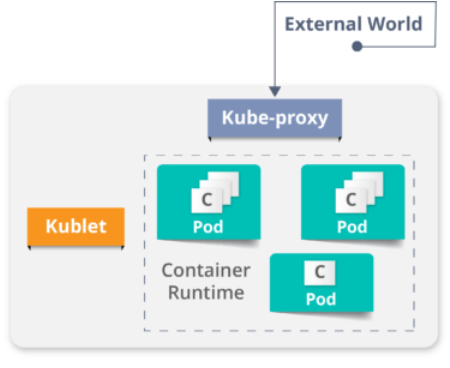
\includegraphics[height=7cm]{images/worker-node}
	\caption{ معماری نود کارگر}
	\label{تصویر 2-12}
\end{figure}

\begin{enumerate}
	\item
	\lr{:container runtime}\\
	جهت اجرای چرخه زمان کانتینرها، نود کارگر به این قسمت نیازمند است. گاهی اوقات داکر به عنوان یک \lr{container runtime}	معرفی می‌شود اما در واقع داکر پلتفرمی می‌باشد که از کانتینرها به عنوان یک \lr{container runtime} استفاده می‌کند. 
	
	\item
	\lr{:Kubelet}\\
	یک عامل است که با نود مستر ارتباط برقرار می‌کند و بر روی نودهای کارگر اجرا می‌شود. همچنین مشخصات فنی پادها را دریافت می‌کند و کانتینرهایی که به پادها مرتبط هستند را اجرا می‌کند. سپس از اجرا و سلامتی کانتیرها اطمینان حاصل می‌کند.
	\item
	\lr{:Kube-proxy}\\
	جهت ارتباط با شبکه (\lr{host sub-netting}) بر روی هر نود اجرا می‌شود و اطمینان حاصل می‌کند که سرویس‌ها برای قسمت‌های خارجی در دسترس هستند. همچنین به عنوان یک پروکسی شبکه و یک  متعادل کننده بار برای سرویس عمل می‌کند و مسیریابی شبکه را برای بسته‌های \lr{TCP} و \lr{UDP} انجام می‌دهد. این پروکسی شبکه دائما به \lr{API server} گوش می‌دهد. برای هر سرویس یک مسیریابی انجام می‌دهد تا بتوان به آن دسترسی داشت.
	\item
	\lr{:Pod}\\
	شامل یک یا چند کانتینر است که کانتینرها از لحاظ منطقی با هم برابرند. پادها به عنوان یک واحد منطقی اجرا می‌شوند. پادها نیاز ندارند که بر روی یک ماشین مجازی اجرا شوند بلکه می‌توان هر کدام را بر روی یک ماشین مجازی متفاوت اجرا کرد. 
\end{enumerate}


\subsubsection{اشیاء کوبرنتیز}

در فضای یک نود کارگر می‌توان از اشیاء\LTRfootnote{object} مختلفی استفاده کرد. اشیاء در کوبرنتیز موجودیت‌های ماندگار هستند. کوبرنتیز از این موجودیت‌ها برای نشان‌دادن حالت و وضعیت خوشه استفاده می‌کند. مهم‌ترین مواردی که این موجودیت‌ها توصیف می‌کنند شامل مشخص‌کردن برنامه‌های کاربردی کانتینر شده در حال اجرا، منابع در دسترس برای برنامه‌های در حال اجرا، سیاست‌هایی که مشخص می‌کند این برنامه‌ها چگونه رفتار کنند و ... می باشد. اشیاء کوبرنتیز یک بار توسط توسعه‌دهنده ایجاد می‌شوند و سیستم کوبرنتیز دائماً این اشیا را زیرنظر می‌گیرد و از وجود آن‌ها اطمینان حاصل می‌کند. با ایجاد یک شی، به سیستم کوبرنتیز می‌گویید که می‌خواهید خوشه چگونه کار کند. بدین ترتیب حالت مورد انتظار خوشه را مشخص می‌کنید. جهت ساخت، اصلاح و یا حذف اشیا نیازمند \lr{kubernetes API} هستید.

هر شیء کوبرنتیز شامل دو قسمت تو‌در‌تو می‌باشد و هر قسمت خود یک شیء است. این دو قسمت تنظیمات شیء را اداره می‌کنند. این دو قسمت \lr{spec} و \lr{status} نام دارند. قسمت \lr{spec} که توسعه‌دهنده باید آن را مهیا کند، حالت مورد انتظار شیء را توصیف می‌کند. قسمت \lr{status} حالت حقیقی و فعلی شیء را توصیف می‌کند که به وسیله سیستم کوبرنتیز تهیه و به‌روز می‌شود.

\newpage

تعدادی از اشیاء کوبرنتیز را معرفی می‌کنیم \cite{sanche_2018}:
\begin{enumerate}
	\item
	\lr{:Pod}\\
	پاد گروهی از یک یا چند کانتینر با انبار ذخیره‌سازی \LTRfootnote{storage} و شبکه به‌اشتراک‌ گذاشته‌ شده می‌باشد. کوبرنتیز به طور مستقیم کانتینرها را اجرا نمی‌کند، بلکه یک یا چند کانتینر را  در ساختاری با نام پاد بسته‌بندی می‌کند. کانتینرهای داخل یک پاد دارای منابع یکسان به همراه شبکه محلی یکسان هستند و به آسانی با دیگر کانتینرهای داخل پاد ارتباط برقرار می‌کنند. این امر به این دلیل است که بر روی یک ماشین قرار دارند. پاد به عنوان واحدی برای تکثیر در کوبرنتیز شناخته می‌شود. اگر استفاده از برنامه کاربردی به اندازه‌ای شود که یک پاد توانایی تحمل بار آن را نداشته باشد، کوبرنتیز می‌تواند به گونه‌ای تنظیم شده باشد که در این حالت پاد موردنظر را تکثیر کند. حتی اگر برنامه‌ زیر بار سنگین نباشد، حالت استاندارد این است که چند کپی از پاد در یک لحظه در حال اجرا باشد تا تعادل بار و کنترل شکست آسان‌تر شود.
	پادها توانایی نگه‌داری چندین کانتینر را دارند اما ترجیح بر آن است که در هر پاد یک کانتینر نگه‌داری شود. چرا که پادها واحدی برای مقیاس‌پذیری هستند در نتیجه در صورت زیاد و یا کم‌ شدن تعداد پادها، همه کانتینرهای داخل پاد با هم زیاد و کم می‌شوند در‌حالی که ممکن است تنها لازم باشد مقیاس یکی از کانتینرها تغییر کند. در نتیجه این امر باعث هدر رفتن منابع و افزایش هزینه‌ها می‌شود. 
	
	\item
	\lr{:Replica set}\\
	یکی از مزایای کلیدی پادها این است که به توسعه‌دهندگان این اجازه را می‌دهند تا مجموعه‌ای از کانتینرها را به عنوان یک برنامه واحد گروه‌بندی و دسته‌بندی کنند و به آسانی با آن‌ها به عنوان یک حجم کار \LTRfootnote{workloads} کار کنند. پس از ساخت پادها، نمونه‌هایی از پادهای ساخته‌شده می‌توانند به صورت افقی مقیاس‌بندی\LTRfootnote{scale} شوند تا برنامه‌های چند کانتینری در دسترس باشند. برای مدیدیت مقیاس‌پذیری پادها، کوبرنتیز از یک \lr{API object} استفاده می‌کند که \lr{replica set} نام دارد.
	بر طبق مستندات کوبرنتیز، \lr{replica set} ها این اطمینان را می‌دهند که تعداد مشخصی از کپی‌های پادها در هر زمان در حال اجرا باشند. 
	در 	\lr{replica set} سه قسمت اصلی وجود دارد (شکل \ref{تصویر 2-15}). قسمت اول \lr{selector} نام دارد. وظیفه این قسمت انتخاب پاد موردنظر جهت مدیریت آن است. قسمت دوم \lr{template}	نام دارد.	\lr{replica set}	با توجه به این قسمت پاد خواسته‌شده ساخته می‌شود. قسمت سوم	\lr{replicas}	نام دارد که تعداد پادهای خواسته‌شده در این قسمت قرار می‌گیرد. با این که	\lr{replica set}	ها توانایی مدیریت پادها را دارند اما قادر به به‌روز‌رسانی متحرک\LTRfootnote{rolling update} نیستند. به همین دلیل از تعریف جدیدی به نام \lr{deployment} استفاده می‌شود \cite{nirmata_ReplicaSetsAndDeployments}.
	
	\begin{figure}[!h]
		\centering
		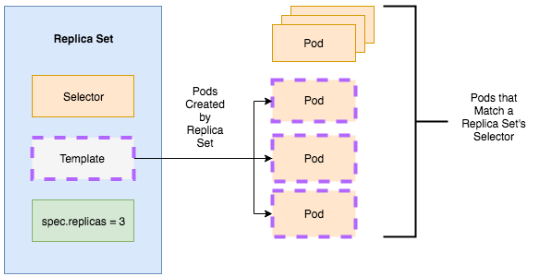
\includegraphics[height=8cm]{images/replicaset}
		\caption{نحوه عملکرد \lr{replica set}}
		\label{تصویر 2-15}
	\end{figure}
	
	\item
	\lr{:Deployment}\\
	با اینکه پادها اساسی‌ترین واحد محاسباتی در کوبرنتیز می‌باشند، اما به صورت مستقیم بر روی خوشه کوبرنتیز راه‌اندازی نمی‌شوند. در عوض پاد‌ها به وسیله‌ی یک لایه انتزاعی به نام \lr{deployment}	مدیریت می‌شوند. هدف اولیه 	\lr{deployment} ها این است که مشخص کنند چند کپی از پاد در یک زمان باید در حال اجرا باشند. وقتی یک \lr{deployment} به خوشه اضافه می‌شود، به صورت اتوماتیک ابتدا تعداد پادهای درخواست‌شده را راه‌اندازی می‌کند سپس بر آن‌ها نظارت می‌کند. اگر یک پاد بمیرد، \lr{deployment} به صورت خودکار دوباره آن را می‌سازد.
	
	از نگاهی دیگر \lr{deployment}، پادها و \lr{replica set} ها را بسته‌بندی می‌کند و روشی اعلامی\LTRfootnote{declarative method} برای به‌روز‌رسانی حالات آن‌ها مهیا می‌کند (شکل \ref{تصویر 2-17}).
	
	\begin{figure}[!h]
		\centering
		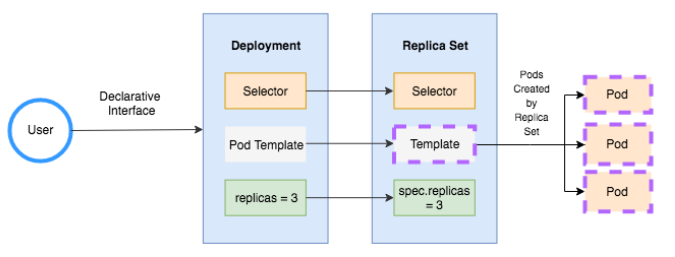
\includegraphics[height=5.5cm]{images/deployment}
		\caption{روش اعلامی ایجاد شده توسط 
			\lr{deployment}
		}
		\label{تصویر 2-17}
	\end{figure}
	
	\item
	\lr{:Service}\\
	یک مفهوم است که مجموعه‌ی منطقی از پادها و سیاست‌های دسترسی به آن‌ها را تعریف می‌کند. \lr{Service} ها یک نقطه پایان\LTRfootnote{endpoint} برای پادها مشخص می‌کنند تا بتوانیم به آن‌ها دسترسی داشته باشیم و بدانیم در چه وضعیتی هستند. 
	\item
	\lr{:Storage class}\\
	راهی برای توصیف کلاس‌های فضای ذخیره توسط مدیران تهیه می‌کند. 
	\item
	\lr{:Persistent Volumes}\\
	اگر یک برنامه اطلاعات خود را در یک فایل محلی در نود ذخیره کند، زمانی که  برنامه به هر دلیلی به نود دیگر انتقال پیدا می‌کند، تضمینی وجود ندارد که اطلاعات در دسترس باشند. به همین علت می‌توان گفت انبارهای ذخیره‌سازی که در نودها وجود دارند به عنوان حافظه‌های موقت عمل می‌کنند و داده‌هایی در آن‌ها جا می‌گیرند پایدار نیستند. برای ذخیره اطلاعات به صورت دائمی کوبرنتیز از \lr{Persistent Volumes} استفاده می‌کند.  \lr{Persistent Volume} ها چرخه حیاتی دارند و مستقل از پادهایی هستند که به آن‌ها متصل می‌شوند.
	
	\item
	\lr{:Persistent Volume Claim}\\
	یک تعریف انتزاعی از \lr{Persistent Volume} می‌باشد. \lr{Persistent Volume} ها منابع فیزیکی زیرساخت‌ها می‌باشند. کوبرنتیز جهت پنهان‌کردن جزییات از توسعه‌دهندگان این مفهوم را استفاده می‌کند. با استفاده از این مفهوم می‌توان تعاریف فیزیکی تعریف‌شده توسط \lr{Persistent Volume}	و \lr{Storage class} را پنهان کرد.
	
	\item
	\lr{:Ingress}\\
	به صورت پیش فرض کوبرنتیز پادها را از محیط بیرون مستقل و ایزوله کرده است. اگر می خواهید کانالی برای ارتباط پادها با فضای بیرون ایجاد کنید از \lr{Ingress} باید استفاده کنید.
\end{enumerate}

\newpage

\section{\lr{OpenWhisk}}

شرکت سرویس های وب آمازون با راه اندازی سرویس بدون سرور خود به اسم \lr{OpenWhisk} در سال ۲۰۱۴ تغییر شگرفی در عرصه رایانش ابری ایجاد کرد. \lr{Lambda} این امکان را به توسعه دهندگان نرم افزار داد که تنها با نوشتن تابع های خود به عنوان کنترل کننده های رویداد بتوانند هزاران رویداد را همزمان پردازش کنند. پس از معرفی \lr{Lambda} گروهی در شرکت \lr{IBM} متوجه ارزش بستر بدون سرور شدند و در سال ۲۰۱۵ تصمیم گرفتند که یک بستر بدون سرور را برای ابر \lr{IBM} طراحی کنند. در ابتدا این بستر "\lr{Whisk}" نام داشت که پس از گذشت یک سال متن باز شد و نام آن به \lr{OpenWhisk} تغییر کرد. اکنون این پروژه قسمتی از \lr{Apache Software Foundation} است و به عنوان اصلی ترین جایگزین متن باز برای \lr{Lambda} حساب می‌شود. محصولات بدون سرور شرکت های \lr{IBM} و \lr{Adobe} با این بستر ساخته شده اند و همچنین بسیاری از شرکت های ارائه دهنده تلفن همراه و اینترنت از آن استفاده می‌کنند.

\lr{OpenWhisk} یک بستر بدون سرور متن باز است که برای آسان کردن توسعه برنامه های کاربردی درون ابر طراحی شده است. برای معرفی و آشنایی بیشتر با این بستر ابتدا با توضیح معماری و ساختارش شروع می‌کنیم و سپس به بررسی نحوه عملکرد قسمت های مختلفش می‌پردازیم.

\subsection{معماری \lr{OpenWhisk}}

همانطور که در شکل \ref{OW-event-action} مشخص است، \lr{OpenWhisk} تابع هایی به اسم \lr{action} را در پاسخ به رویدادها اجرا می‌کند. این رویدادها می‌توانند توسط تایمرها، پایگاه داده‌ها، صف‌های پیام و یا وبسایت‌های مختلف تولید شده باشند. \lr{OpenWhisk} کد منبع را با رابط خط فرمان (\lr{CLI}) ورودی می‌گیرد و سرویس های خود را از راه  شبکه اینترنت به مصرف کننده های مختلف مانند وب سایت ها، برنامه های کاربردی تلفن همراه و یا سرویس های \lr{REST API} ارائه می‌دهد. 
\begin{figure}[!h]
	\centering
	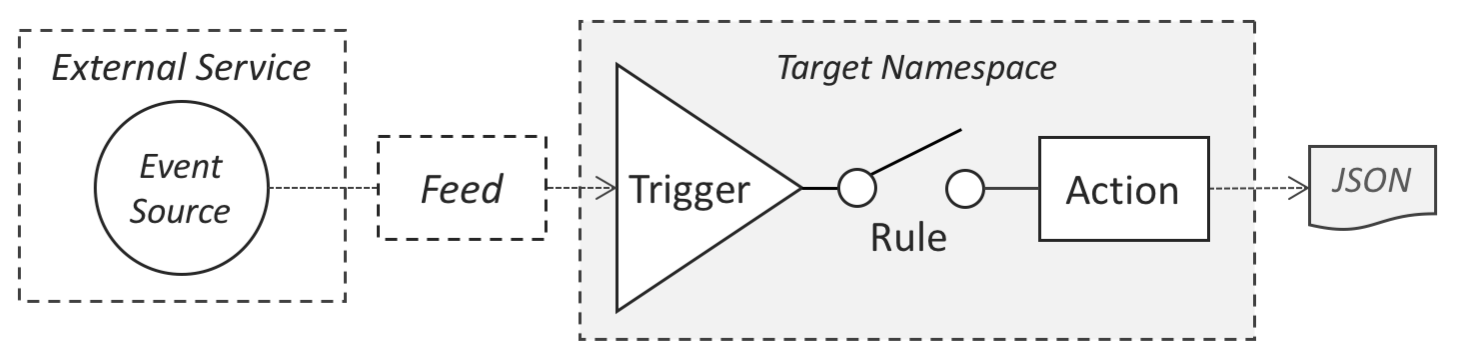
\includegraphics[height=4cm]{images/OW-event-action}
	\caption{نحوه‌ی عملکرد رویداد محور \lr{OpenWhisk}}
	\label{OW-event-action}
\end{figure}

\subsection{تابع‌ها و رویدادها}

\lr{OpenWhisk} با اجرا کردن تابع ها کارها را انجام می‌دهد. تابع تکه‌ای از کد است که چند ورودی دریافت و در پاسخ یک خروجی تولید می‌کند. یک تابع به طور کلی وضعیت را نگه نمی‌دارد (\lr{stateless})، اما برنامه های کاربردی که سمت سرور اجرا می‌شوند (‌\lr{backend}) وضعیت را کاملاً حفظ می‌کنند (\lr{stateful}). حفظ کردن وضعیت، مقیاس پذیری را محدود می‌کند زیرا در مقیاس های بالا به فضای خیلی زیادی برای نگهداری داده ها نیاز است. مهم تر از آن به سیستمی‌نیاز است که وضعیت بین فراخوانی‌های مختلف را همگام سازی کند. در نتیجه با افزایش بار سرور، زیرساخت عملیات حفظ و همگام‌سازی وضعیت تبدیل به مانعی در برابر رشد پروژه می‌شود. حفظ نکردن وضعیت اما این مزیت را دارد که می‌توان به راحتی چندین سرور دیگر را برای پروژه به کار گرفت بدون این که نیازی به همگام سازی وضعیتشان باشد.

در \lr{OpenWhisk} و به طور کلی در محیط بدون سرور تابع ها نباید وضعیت را نگهداری کنند. در محیط بدون سرور می‌توان وضعیت را نگهداری کرد اما نه در سطح یک تابع. برای نگهداری وضعیت باید از محل‌های ذخیره‌سازی مخصوصی استفاده شود که دارای قابلیت مقیاس پذیری بالا هستند.

\lr{OpenWhisk} زیرساخت را مدیریت می‌کند و آن را برای رخ دادن اتفاق مهمی آماده نگه می‌دارد. این اتفاق مهم رویداد\LTRfootnote{event} نام دارد. تنها در صورتی یک تابع فراخوانی و اجرا می‌شود که رویدادی رخ داده باشد. این پردازش رویدادها در واقع مهم ترین عملیاتی است که محیط بدون سرور آن را مدیریت می‌کند. در نتیجه توسعه دهنده ها تنها باید برنامه ای بنویسند که به این رویدادها به طرز صحیحی پاسخ دهد و بقیه کارها به عهده ی ارائه دهنده ی سرویس می‌باشد.

\subsection{زبان های برنامه نویسی \lr{OpenWhisk}}

\lr{action} های \lr{OpenWhisk} را می‌توان با بسیاری از زبان های برنامه نویسی نوشت. اما معمولاً از زبان های تفسیر شده\LTRfootnote{interpreted} استفاده می‌شود، مانند \lr{JavaScript}، \lr{Python} یا \lr{PHP}. این زبان های برنامه نویسی به دلیل اجرا پذیر بودن بدون نیاز به کامپایل، در بازخورد طراحی خیلی سریع هستند. همچنین چون جزو زبان های سطح بالا محسوب می‌شوند، استفاده از آن ها نیز راحت تر است، اما در اجرا کندتر از زبان های کامپایل شده هستند.

علاوه بر زبان های تفسیر شده می‌توان از زبان های تفسیر شده ی از قبل کامپایل شده مانند \lr{Java} و \lr{Scala} استفاده کرد. این زبان ها توسط ماشین مجازی \lr{Java} یا به اختصار \lr{JVM} اجرا می‌شوند.

در نهایت از زبان های کامپایل شده نیز در \lr{OpenWhisk} می‌توان استفاده کرد. در این حالت یک فایل باینری اجراپذیر بر روی سیستم بدون هیچ واسطه‌ای اجرا می‌شود. \lr{OpenWhisk} تنها از زبان های \lr{Go} و \lr{Swift} در این دسته از زبان ها پشتیبانی می‌کند.

به جز زبان های گفته شده از هر نوع زبان و سیستمی نیز برای تعریف \lr{action} های \lr{OpenWhisk} می‌توان استفاده کرد به این شرط که به عنوان یک ایمیج داکر بسته بندی شود و در \lr{Docker hub} منتشر شود. \lr{OpenWhisk} می‌تواند با دریافت ایمیج، آن را اجرا کند.

\subsection{\lr{Action} ها}

برنامه های ساخته شده با \lr{OpenWhisk} مجموعه ای متشکل از \lr{action} ها هستند. این \lr{action} ها تکه ای کد هستند که با زبان های گفته شده نوشته شده اند و می‌توان آن ها را فراخوانی و اجرا کرد (\lr{invoke}). در زمان فراخوانی \lr{action}، تعدادی ورودی با فرمت \lr{JSON} به تابع آن داده می‌شود. سپس در انتهای اجرا، \lr{action} باید یک خروجی تولید کند که آن هم نیز باید با فرمت \lr{JSON} بازگشت داده شود.

\lr{action} ها را می‌توان با استفاده از \lr{package} ها دسته بندی نمود. یک \lr{package} را می‌توان به وسیله \lr{binding} ها با بقیه \lr{user} ها به اشتراک گذاشت. همچنین برای یک \lr{package} می‌توان مؤلفه هایی تعیین کرد که مختص هر \lr{binding} باشند و به \lr{action} هایش به ارث برسند.

\subsection{زنجیر کردن \lr{Action} ها}

\lr{action} ها از راه های مختلفی می‌توانند به یکدیگر متصل شوند. ساده ترین راه متصل کردن به وسیله \lr{sequence} است. \lr{action} های متصل به هم از خروجی \lr{action} قبل از خود به عنوان ورودی استفاده می‌کنند.

بسیاری از جریان‌های مورد نیاز برای پیاده‌سازی منطق برنامه را نمی‌توان به صورت یک مسیر خطی تعریف کرد که تنها یک ورودی می‌گیرند و در انتها یک خروجی را برمی‌گردانند. بنابراین راهی وجود دارد که می‌توان جریان \lr{action} ها را به مسیرهای مختلف تقسیم کرد. این ویژگی با \lr{trigger} ها (ماشه ها) و \lr{rule} ها (قوانین) پیاده‌سازی می‌شود. یک \lr{trigger} به تنهایی کاری انجام نمی‌دهد، اگرچه می‌توان آن را با یک یا چند \lr{action} از طریق تعریف کردن \lr{rule} مرتبط کرد. پس از تعریف کردن \lr{trigger} و مرتبط کردن آن با چندین \lr{action} می‌توان آن را با دادن مؤلفه‌ها شلیک (\lr{fire}) کرد. در شکل \ref{OpenWhisk_actions_architecture} معماری \lr{action} های \lr{OpenWhisk} نشان داده شده است.
\newline
\newline

\begin{figure}[!h]
	\centering
	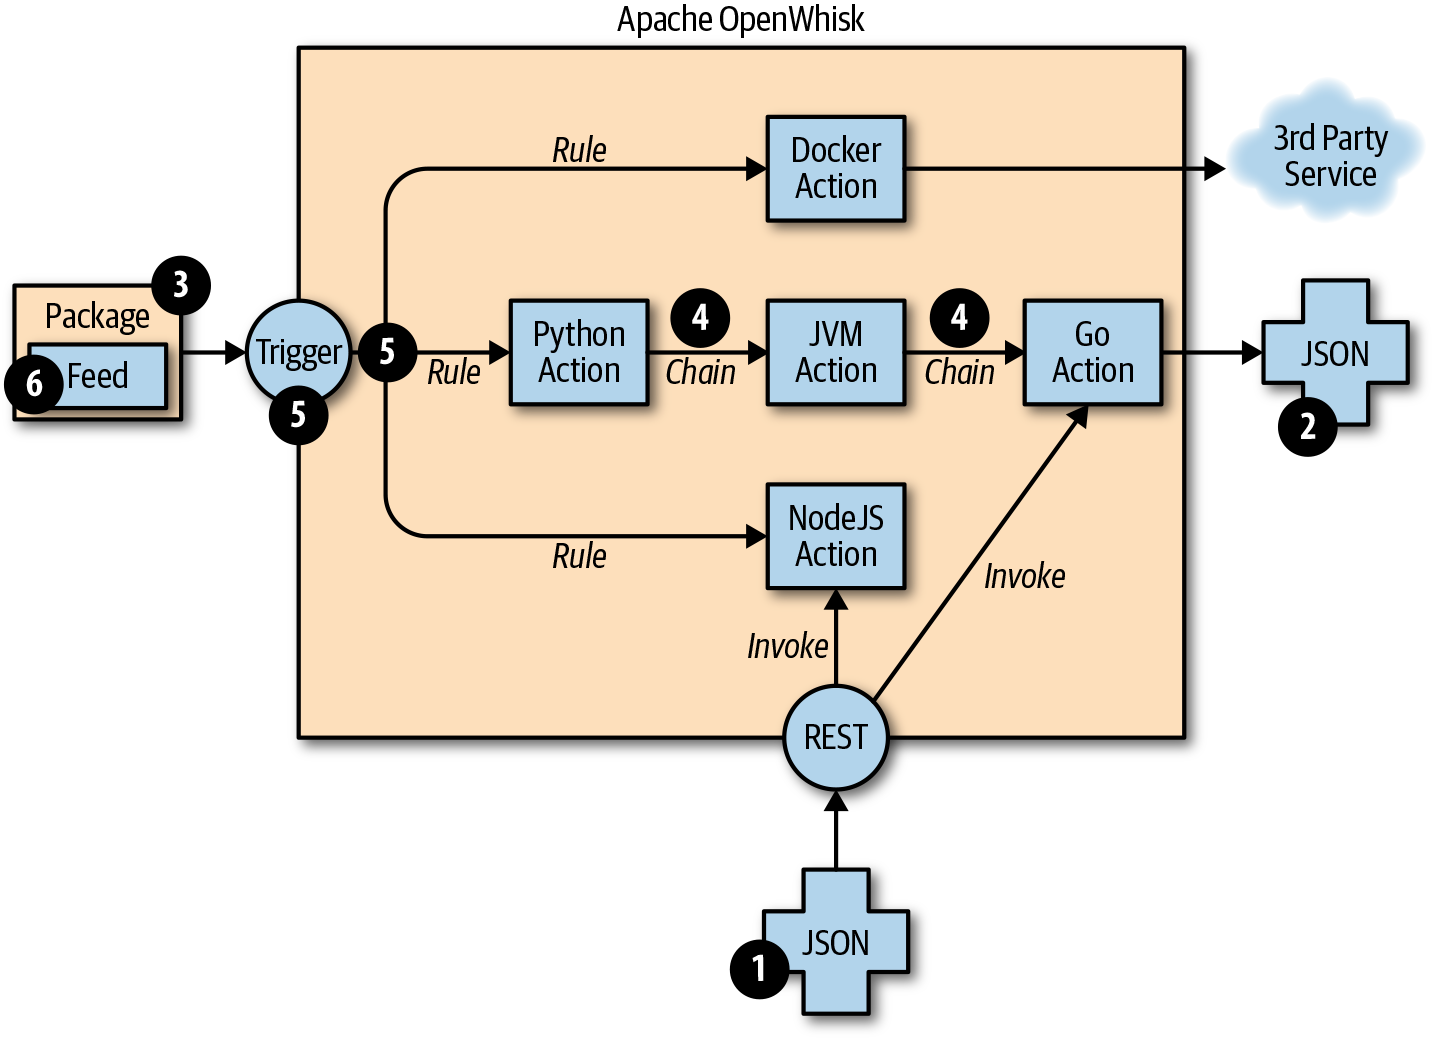
\includegraphics[height=11cm]{images/OpenWhisk_actions_architecture}
	\caption{نمای کلی ساختار \lr{action} های \lr{OpenWhisk}}
	\label{OpenWhisk_actions_architecture}
\end{figure}

برای شلیک کردن \lr{trigger} یک \lr{action} باید تعریف کرد که \lr{feed} نام دارد. \lr{feed} باید طبق الگوی طراحی ناظر\LTRfootnote{observer} طراحی شود و بتواند یک \lr{trigger} را در هنگام رخ دادن یک رویداد فعال کند. الگوی ناظر یک الگوی طراحی نرم‌افزار است که در آن یک شی به نام موضوع، فهرست وابستگی‌هایش را با نام ناظران نگه می‌دارد و هرگونه تغییر در وضعیتش را به‌طور خودکار و معمولاً با صدا کردن یکی از روش‌های آن به اطلاع آن اشیا می‌رساند. پس از طراحی \lr{feed} در هنگام پیاده‌سازی برنامه می‌توان آن را با یک \lr{trigger} ادغام نمود تا آن \lr{trigger} نیز در هنگام شلیک، چند \lr{action} دیگر را فراخوانی کند.

\newpage

\subsection{نحوه عملکرد \lr{OpenWhisk}}

حال پس از آشنایی با اجزاء مختلف \lr{OpenWhisk} به بررسی نحوه عملکرد آن‌ها می‌پردازیم.

\lr{OpenWhisk} با بهره‌گیری از چندین پروژه معروف و توسعه یافته متن باز ساخته شده است که در زیر معرفی شده اند: (شکل \ref{OpenWhisk_flow_of_processing})

\textbf{\lr{Nginx}} : یک وب سرور با کارایی بالا و پروکسی معکوس

\textbf{\lr{CouchDB}} : پایگاه داده سند محور، \lr{NoSQL} و مقیاس پذیر

\textbf{\lr{Kafka}} : سیستم پیام رسانی انتشار-اشتراک توزیع شده با کارایی بالا و مقیاس پذیر

تمامی‌این اجزاء کانتینرهای داکر هستند و می‌توانند توسط محیط‌هایی که از این فرمت پشتیبانی می‌کنند مانند کوبرنتیز اجرا شوند.
\newline

\lr{OpenWhisk} شامل قسمت های دیگری می‌باشد که توسط تیم خودش ساخته شده است:

\textbf{\lr{Controller}} : موجودیت های مختلف را مدیریت می‌کند، \lr{trigger} ها را شلیک می‌کند و همچنین فراخوانی \lr{action} ها را مسیریابی می‌کند.

\textbf{\lr{Invoker}} : کانتینرها را برای اجرای \lr{action} ها راه اندازی می‌کند.

\textbf{\lr{Action containers}} : کانتینرهای حاوی \lr{action} که در واقع \lr{action} ها را اجرا می‌کنند.

\begin{figure}[!h]
	\centering
	\includegraphics[height=9cm]{images/OpenWhisk_flow_of_processing}
	\caption{ساختار \lr{OpenWhisk}}
	\label{OpenWhisk_flow_of_processing}
\end{figure}

\newpage

تمامی‌پردازشی که در \lr{OpenWhisk} انجام می‌شود ناهمگام\LTRfootnote{asynchronous} است. این پردازش شامل دریافت، کنترل، صف‌بندی، پردازش و ذخیره‌سازی نتایج یک درخواست فراخوانی \lr{action} است. حال با جزئیات بیشتری به بررسی این مراحل می‌پردازیم. نمودار زمانی این مراحل در شکل \ref{action_invokation_timeline} نشان داده شده است.

\begin{figure}[!h]
	\centering
	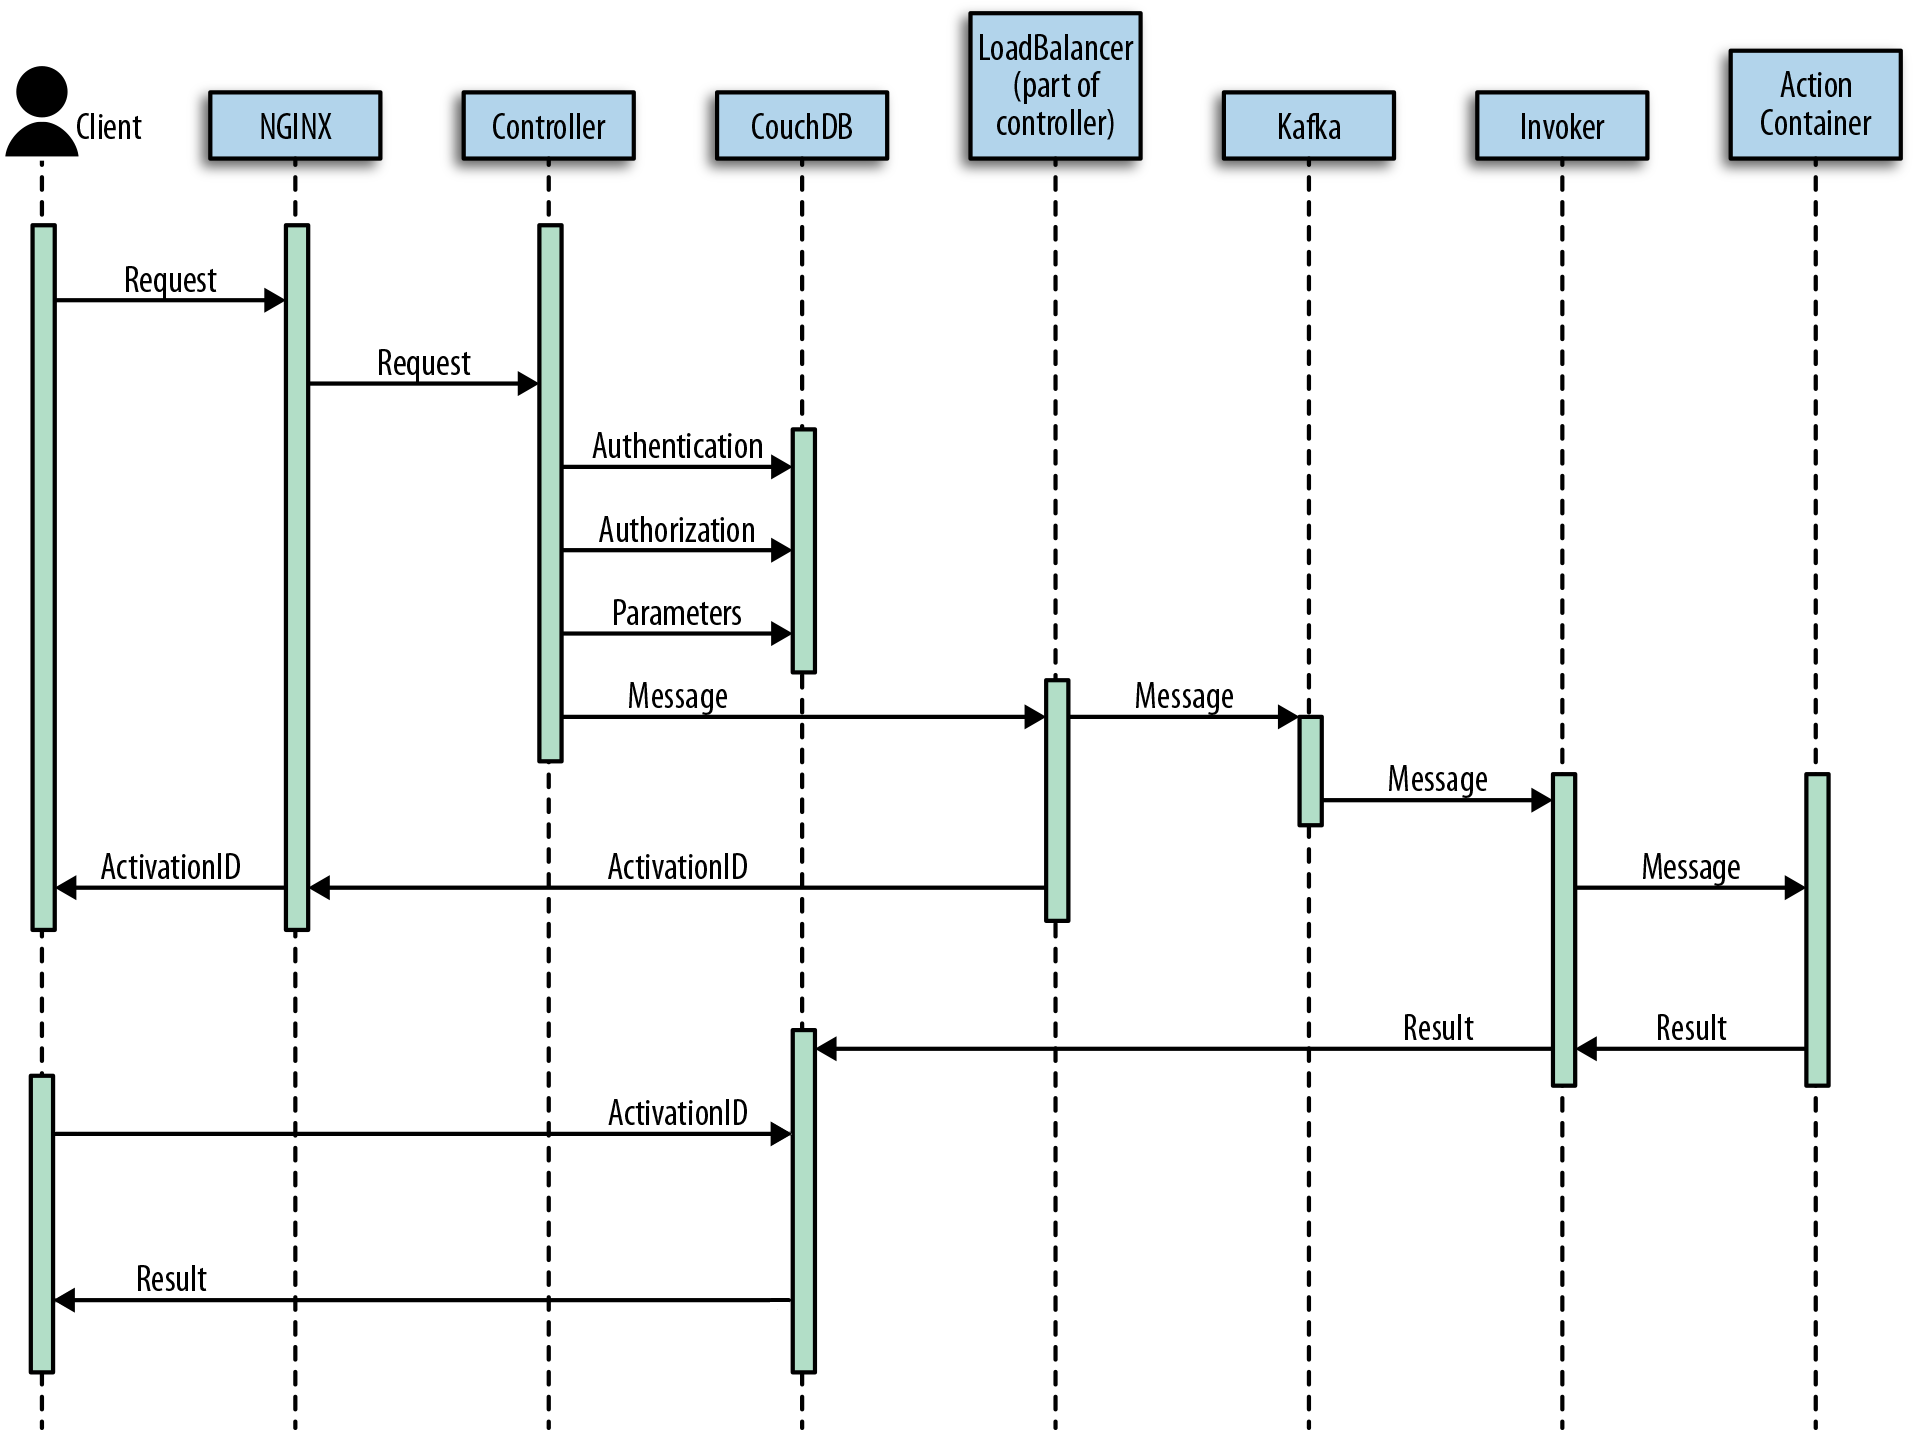
\includegraphics[height=12cm]{images/action_invokation_timeline}
	\caption{چگونگی پردازش \lr{action} در \lr{OpenWhisk}}
	\label{action_invokation_timeline}
\end{figure}

\subsubsection*{\lr{Nginx}}

همه چیز با فراخوانی \lr{action} آغاز می‌شود. این فراخوانی از راه های مختلفی امکان پذیر است:

\begin{itemize}

	\item از طریق وب هنگامی‌که \lr{action} به عنوان \lr{web action} تعریف شده باشد.
	
	\item فراخوانی از \lr{action} دیگر با استفاده از \lr{API}
	
	\item هنگامی‌که یک \lr{trigger} فعال شود و یک \lr{rule} برای فراخوانی \lr{action} وجود داشته باشد.
	
	\item از طریق \lr{CLI}
	
\end{itemize}

\lr{OpenWhisk} یک سیستم \lr{RESTful} است، بنابراین هر فراخوانی \lr{action} به یک درخواست \lr{HTTPS} تبدیل می‌شود و به نود‌ی لبه که همان \lr{Nginx} است می‌رسد. دلیل اصلی وجود وب سرور \lr{Nginx}، پیاده‌سازی و پشتیبانی از پروتکل امن \lr{HTTPS} می‌باشد. \lr{Nginx} پس از دریافت درخواست آن را به سرویس اصلی میانی به نام \lr{Controller} می‌فرستد.

\subsubsection*{\lr{Controller}}

قبل از اجرا شدن \lr{action}، ابتدا \lr{controller} امکان اجرای و صحت آن را بررسی می‌کند. سپس منبع آن هویت سنجی می‌شود تا اجازه دسترسی آن مشخص شود. اگر \lr{action} از دو مرحله قبل عبور کرد، مؤلفه های اضافی به عنوان پیکربندی به آن افزوده می‌شود. حال که امکان اجرای \lr{action} تأیید شد، به قسمت بعدی که \lr{Load Balancer} است فرستاده می‌شود.

\subsubsection*{\lr{Load Balancer}}

وظیفه ی \lr{Load Balancer} همان طور که از نامش پیداست حفظ تعادل میان اجرا کننده های \lr{action} یا همان \lr{invoker} های \lr{OpenWhisk} است. \lr{Load Balancer} با مواظبت از \lr{runtime} های \lr{action} موجود، اگر دوباره مورد نیاز باشد از آن استفاده می‌کند و اگر \lr{runtime} مورد نیاز موجود نبود آن را می‌سازد.

\subsubsection*{\lr{Kafka}}

به جایی رسیدیم که سیستم آماده اجرای \lr{action} است. با این حال، نمی‌توان آن \lr{action} را فوراً به یک \lr{invoker} ارسال کرد، زیرا ممکن است مشغول اجرای یک \lr{action} دیگر باشد. همچنین این احتمال وجود دارد که یک \lr{invoker} خراب شود، یا حتی کل سیستم خراب شده و دوباره راه اندازی شود. بنابراین، از آنجا که ما در یک محیط کاملاً موازی کار می‌کنیم که انتظار می‌رود مقیاس پذیر باشد ، باید این احتمال را در نظر بگیریم که منابع مورد نیاز خود را برای اجرای فوری \lr{action} در دسترس نداشته باشیم. در مواردی از این دست، مجبوریم فراخوانی ها را بافر کنیم. \lr{OpenWhisk} از \lr{Kafka} برای انجام این عمل استفاده می‌کند. \lr{Kafka} یک سیستم پیام رسان "انتشار - اشتراک" با عملکرد بالا است که می‌تواند درخواست ها را تا زمان آماده شدن برای اجرای آن ها ذخیره کند. درخواست که برای ورود به \lr{Nginx} به \lr{HTTPS} تبدیل شده بود، توسط \lr{Load Balancer} به یک پیام \lr{Kafka} تبدیل می‌شود که به \lr{invoker} مقصدش آدرس دهی شده است.

هر پیام ارسال شده به یک \lr{invoker} شناسه ای دارد به نام \lr{activation-ID}. هنگامی‌که پیام در صف \lr{Kafka} قرار می‌گیرد، دو امکان وجود دارد: فراخوانی بدون انسداد و مسدود کننده. برای یک فراخوانی بدون انسداد‌، شناسه فعال سازی به عنوان پاسخ نهایی درخواست به \lr{client} ارسال می‌شود و درخواست تکمیل می‌شود. در این حالت ، پیش بینی می‌شود \lr{client} بعداً برگردد تا نتیجه فراخوانی را بررسی کند. برای یک فراخوانی مسدود کننده، اتصال باز می‌ماند؛ کنترل کننده منتظر نتیجه \lr{action} است و نتیجه را برای سرویس‌گیرنده ارسال می‌کند.

\subsubsection*{\lr{Invoker}}

در \lr{OpenWhisk}، بخش \lr{invoker} وظیفه اجرای \lr{action} را بر عهده دارد. \lr{action} ها در واقع در محیط های جدا شده که توسط کانتیرهای \lr{Docker} ساخته شده اند، اجرا می‌شوند به این صورت که \lr{invoker} ابتدا ایمیج \lr{runtime} مورد نیاز برای اجرای \lr{action} را انتخاب می‌کند و سپس آن را همراه با کد \lr{action} راه اندازی می‌کند.

پس از اینکه \lr{runtime} اجرا شد، \lr{action} هایی که تا آن زمان ساخته و آماده شده اند توسط \lr{invoker} به \lr{runtime} فرستاده می‌شوند. \lr{invoker} همچنین \lr{log} هایی که مربوط به اجرای \lr{action} ها هستند را مدیریت و ذخیره می‌کند.

\subsubsection*{\lr{CouchDB}}

پس از اتمام پردازش، \lr{OpenWhisk} نتیجه را در پایگاه داده \lr{CouchDB} ذخیره می‌کند. سپس تمامی نتایج اجرای \lr{action} ها که در پایگاه داده ذخیره شده‌اند توسط \lr{activation-ID} که به \lr{client} ارسال شده بود، در دسترس هستند.

\subsubsection*{\lr{Client}}

پردازشی که اکنون توضیح داده شد ناهمگام بود. بدان معنی که سرویس‌گیرنده درخواستی را آغاز می‌کند و سپس آن را کنار می‌گذارد، اگرچه آن را به طور کامل فراموش نمی‌کند، زیرا یک شناسه فعال‌سازی را به عنوان نتیجه‌ی فراخوانی دریافت کرده است. از \lr{activation-ID} برای ذخیره نتیجه در پایگاه داده پس از پردازش استفاده می‌شود. برای بازیابی نتیجه نهایی، سرویس‌گیرنده باید درخواست دیگری را همراه با شناسه فعال سازی به عنوان مؤلفه ورودی ارسال کند. پس از اتمام \lr{action}، نتیجه، \lr{log} ها و سایر اطلاعات در پایگاه داده موجود است و قابل بازیابی است. پردازش همگام هم امکان پذیر است که مانند همان روش پردازش ناهمگام کار می‌کند، اما مسدود کننده است به این معنی که سرویس‌گیرنده منتظر اجرای کامل \lr{action} می‌ماند و نتیجه را فوراً دریافت می‌کند \cite{sciabarrà_michele_2019}.
